\documentclass[10pt]{llncs}


%\usepackage{mathtools}
%\usepackage{makecell}
%\usepackage[]{graphics}
\usepackage[table]{xcolor}
\usepackage{tikz}

%\usepackage{cuted}
%\usepackage[dvipdfmx]{graphicx}
% \graphicspath{ {./images/} }

\usepackage{amsmath}
\usepackage{pdflscape}
\usepackage{rotating}
\usepackage{authblk}
\usepackage{appendix}
\usepackage{colortbl}
% \usepackage[top=0.85in,left=2.75in,footskip=0.75in]{geometry}
%\allowdisplaybreaks{}

%\expandafter\def\csname ver@etex.sty\endcsname{3000/12/31}
%\let\globcount\newcount

% I ADDED FOR THE CHANGE IN ENUMERATE TO ALPHABBETICAL
% \usepackage{enumitem}

%\DeclareFontShape{OT1}{cmr}{bx}{sc}{<-> cmbcsc10}{}

% amsmath and amssymb packages, useful for mathematical formulas and symbols
\usepackage{amsmath,amssymb}

% \renewcommand{\figurename}{Fig.{}}

% Use adjustwidth environment to exceed column width (see example table in text)
% \usepackage{changepage}

% Use Unicode characters when possible
% \usepackage[utf8x]{inputenc}

% textcomp package and marvosym package for additional characters
\usepackage{textcomp,marvosym}

% cite package, to clean up citations in the main text. Do not remove.
% \usepackage{cite}

% Use nameref to cite supporting information files (see Supporting Information section for more info)
\usepackage{nameref,hyperref}

% line numbers
% \usepackage[right]{lineno}
% \linenumbers
% ligatures disabled
%\usepackage{microtype}
%\DisableLigatures[f]{encoding = *, family = * }

% color can be used to apply background shading to table cells only
\usepackage{xargs}                      % Use more than one optional parameter in a new commands
% \usepackage[pdftex,dvipsnames,table]{xcolor}  % Coloured text etc.
%\usepackage{todonotes}

% array package and thick rules for tables
\usepackage{array}

% Use package Listing to add code in our Manuscript
\usepackage{listings} 

%\usepackage[figurename=Fig]{caption}
% Added for the sub-pictures
\usepackage{subcaption}

% Added for the multi-column 
\usepackage[british]{babel}
\usepackage{hhline}
\usepackage{multirow}

% Packages for algorithm
\usepackage{algorithmicx}
\usepackage[noend]{algpseudocode}
\usepackage{algorithm}
\usepackage{diagbox}
\algdef{SE}[DOWHILE]{Do}{doWhile}{\algorithmicdo}[1]{\algorithmicwhile\ #1}%

%ADEDED BY ANKIT
% use (a) and i in the enumerate
% \usepackage{enumitem}
% %\usepackage[outdir=./images/]{epstopdf}
% %% Save the class definition of \subparagraph
% \let\llncssubparagraph\subparagraph
% %% Provide a definition to \subparagraph to keep titlesec happy
% \let\subparagraph\paragraph
% %% Load titlesec
% % \usepackage[compact]{titlesec}
% %% Revert \subparagraph to the llncs definition
% \let\subparagraph\llncssubparagraph

%\titlespacing\section{0pt}{12pt plus 4pt minus 2pt}{0pt plus 2pt minus 2pt}
%\titlespacing{\section}{0pt}{*5}{*1.5}
%\titlespacing{\subsection}{0pt}{*4}{*1.5}
%\titlespacing\subsection{0pt}{12pt plus 4pt minus 2pt}{0pt plus 2pt minus 2pt}
%\titlespacing\subsubsection{0pt}{12pt plus 4pt minus 2pt}{0pt plus 2pt minus 2pt}


%Adjust the table 
\usepackage{adjustbox}


%add label refernce from another doc
\usepackage{xr}
\usepackage{catchfilebetweentags}

\usepackage{tkz-orm}
\usetikzlibrary{arrows,shapes,automata,backgrounds,petri,decorations.markings}
\usetikzlibrary{matrix,positioning,decorations.pathreplacing,calc,tikzmark}

\tikzset{
  ln/.style  = { draw, thick, fill=black, circle, inner sep=0.3mm},
  sqloc/.style  = { draw, thick, inner sep=1.0mm },
  loc/.style    = { draw, circle, thick, inner sep=1.0mm },
  notice/.style= { draw, rectangle callout, thick, rounded corners=5pt,fill=blue!10,callout relative pointer={#1} },
  treenode/.style = {align=center, inner sep=0pt, text centered,
    font=\sffamily},
  arn_n/.style = {treenode, rectangle, font=\sffamily\bfseries },% arbre rouge noir, noeud noir
  mymat/.style = { % matrix of math nodes,
    left delimiter={[}, right delimiter ={]},nodes={anchor=base east} },
  align at top/.style={baseline=(current bounding box.north)},
  stack/.style={rectangle split, rectangle split parts=#1,draw, anchor=center}
}

\def\fsmt{\mathsf{SMT}}
\def\fbmc{\mathsf{BMC}}
\def\fqbf{\mathsf{QBF}}

%\usepackage{lineno}
%\linenumbers

\usepackage{verbatim}
\usepackage{pgfplots}
%\usepackage{colortbl}
%\usepackage{pgfplotstable}
% \pgfplotsset{compat=1.17}
	
\def\cca#1{\cellcolor{blue!#10}\ifnum #1>5\color{white}\fi{#1}}

\usepackage{tikz}
\usetikzlibrary{tikzmark,decorations.pathreplacing,arrows,shapes,positioning,shadows,trees,shapes.gates.logic.US,arrows.meta,shapes,automata,petri,calc}
\usepackage{caption}
\usepackage{adjustbox}
%\usepackage{todonotes}
\usepackage[colorinlistoftodos,prependcaption,textsize=tiny]{todonotes}
\newcommandx{\unsure}[2][1=]{\todo[linecolor=red,backgroundcolor=red!25,bordercolor=red,#1]{#2}}
\newcommandx{\change}[2][1=]{\todo[linecolor=blue,backgroundcolor=blue!25,bordercolor=blue,#1]{#2}}
\newcommandx{\info}[2][1=]{\todo[linecolor=OliveGreen,backgroundcolor=OliveGreen!25,bordercolor=OliveGreen,#1]{#2}}
\newcommandx{\improve}[2][1=]{\todo[linecolor=Plum,backgroundcolor=Plum!25,bordercolor=Plum,#1]{#2}}
\usepackage{verbatim}
\usepackage{scalefnt}
\usepackage{wrapfig}
\usepackage{tikz-qtree}
% \usepackage[table, dvipsnames]{xcolor}

\mathchardef\mhyphen="2D
\newcommand{\shorteq}{%
  \settowidth{\@tempdima}{-}% Width of hyphen
  \resizebox{\@tempdima}{\height}{=}%
}


%\definecolor{ai}{RGB}{179, 255, 179}
%\colorlet{fv}{red!55}
%\colorlet{ai}{blue!10}
%\colorlet{ar}{green!56}

\colorlet{fv}{gray!55}
\colorlet{ai}{gray!10}
\colorlet{ar}{gray!38}

\usepackage[edges]{forest}
\usepackage[T1]{fontenc}
% \usepackage{lmodern}

\tikzset{%
  parent/.style={align=center,text width=3cm,rounded corners=3pt},
  child/.style={align=center,text width=3cm,rounded corners=3pt},
}

% argument #1: any options
\newenvironment{customlegend}[1][]{%
	\begingroup
	% inits/clears the lists (which might be populated from previous
	% axes):
	\csname pgfplots@init@cleared@structures\endcsname
	\pgfplotsset{#1}%
}{%
	% draws the legend:
	\csname pgfplots@createlegend\endcsname
	\endgroup
}%
\def\addlegendimage{\csname pgfplots@addlegendimage\endcsname}

\newcommand*{\equal}{=}
 \usepackage{tikz}
% \usetikzlibrary{arrows}
 \usepackage{xparse}
%\usetikzlibrary{}
\pgfdeclarelayer{myback}
\pgfsetlayers{myback,background,main}
\usetikzlibrary{tikzmark,decorations.pathreplacing,arrows,shapes,positioning,shadows,trees,shapes.gates.logic.US,arrows.meta,shapes,automata,petri,calc,matrix,backgrounds}
\tikzset{mycolor/.style = {line width=1bp,color=#1}}%
\tikzset{myfillcolor/.style = {draw,fill=#1}}%


\NewDocumentCommand{\highlight}{O{blue!40} m m}{%
\draw[mycolor=#1] (#2.north west)rectangle (#3.south east);
}

\NewDocumentCommand{\fhighlight}{O{blue!40} m m}{%
\draw[myfillcolor=#1] (#2.north west)rectangle (#3.south east);
}
 \usetikzlibrary{matrix,decorations.pathreplacing, calc, positioning}



% create "+" rule type for thick vertical lines
\newcolumntype{+}{!{\vrule width 2pt}}
\renewcommand{\thesubfigure}{\Alph{subfigure}}

% create \thickcline for thick horizontal lines of variable length
\newlength\savedwidth
\newcommand\thickcline[1]{%
  \noalign{\global\savedwidth\arrayrulewidth\global\arrayrulewidth 2pt}%
  \cline{#1}%
  \noalign{\vskip\arrayrulewidth}%
  \noalign{\global\arrayrulewidth\savedwidth}%
}

\usepackage{array}
\newcolumntype{L}[1]{>{\raggedright\let\newline\\\arraybackslash\hspace{0pt}}m{#1}}
\newcolumntype{C}[1]{>{\centering\let\newline\\\arraybackslash\hspace{0pt}}m{#1}}
\newcolumntype{R}[1]{>{\raggedleft\let\newline\\\arraybackslash\hspace{0pt}}m{#1}}


% Remove comment for double spacing
%\usepackage{setspace} 
%\doublespacing

% Text layout
% \raggedright
% \setlength{\parindent}{0.5cm}
% \textwidth 5.25in 
% \textheight 8.75in
% create "+" rule type for thick vertical lines
% \newcolumntype{+}{!{\vrule width 2pt}}
\renewcommand{\thesubfigure}{\Alph{subfigure}}

% \thickhline command for thick horizontal lines that span the table
\newcommand\thickhline{\noalign{\global\savedwidth\arrayrulewidth\global\arrayrulewidth 2pt}%
\hline
\noalign{\global\arrayrulewidth\savedwidth}}

% \raggedright
% \setlength{\parindent}{0.5cm}
% \textwidth 5.25in 
% \textheight 8.75in


% \usepackage[aboveskip=1pt,labelfont=bf,labelsep=period,justification=raggedright,singlelinecheck=off]{caption}
% \renewcommand{\figurename}{Fig}
% \usepackage{epstopdf}
% \AppendGraphicsExtensions{.tif}

\newcommand{\booleans}{\mathbb{B}}
\newcommand{\naturals}{\mathbb{N}}
\newcommand{\integers}{\mathbb{Z}}
\newcommand{\ordinals}{\mathbb{O}}
\newcommand{\numarals}{\mathbb{I}}
\newcommand{\reals}{\mathbb{R}}

\newcommand{\maps}{\rightarrow}
\newcommand{\pmaps}{\hookrightarrow}

\newcommand{\union}{{\cup} }
\newcommand{\Union}{{\bigcup} }
\newcommand{\powerset}[1]{2^{#1}}
\newcommand{\intersection}{{\cap} }
\newcommand{\intersect}{\intersection}
\newcommand{\Intersection}{{\bigcap} }
\newcommand{\compose}{{\circ} }


\newcommand{\ltrue}{\mathbf{tt}}
\newcommand{\lfalse}{\mathbf{ff}}
\newcommand{\limplies}{\Rightarrow}
\newcommand{\lxor}{\oplus}
\newcommand{\Land}{\bigwedge}
\newcommand{\Lor}{\bigvee}
\newcommand{\Lxor}{\bigoplus}
\newcommand{\lequiv}{\Leftrightarrow}
\newcommand{\landplus}{\mathrel{:\hspace{-3pt}\land\hspace{-3pt}=}}
\newcommand{\lorplus}{\mathrel{:\hspace{-3pt}\lor\hspace{-3pt}=}}

\newcommand{\nodes}{\mathcal{N}}
\newcommand{\mols}{M}
\newcommand{\nlabel}{L}
\newcommand{\edges}{E}
\newcommand{\pairs}{\mathcal{P}}
\newcommand{\nodef}{f}
\newcommand{\edgef}{g}

\newcommand*{\var}{Var}
\newcommand{\wff}{$\mathcal{W}$} % choose suitable symmbol
\newcommand*{\ltf}{\mathcal{F}} % choose suitable symmbol
\newcommand*{\prop}{\mathcal{P}}
\newcommand*{\op}{\mathcal{O}}
\newcommand*{\Next}{\textsf{X}}
\newcommand*{\until}{\textsf{\,U\,}}
\newcommand*{\finally}{\textsf{F}}
\newcommand*{\globally}{\textsf{G}}
\newcommand*{\val}{V(\varphi, w)}
\newcommand*{\sample}{\mathcal{S}}

\newcommand{\varpsi}{\psi}

\newcommand{\depth}{\ensuremath{d}}
\newcommand{\discount}{\ensuremath{\delta}}


\newcommand{\lorem}{{\bf LOREM}}
\newcommand{\ipsum}{{\bf IPSUM}}

\newcommand{\npath}{\texttt{NPath}}

\newcommand{\vtstool}{\textsc{VTSArch}}
\newcommand{\zthree}{\textsc{Z3}}
\newcommand{\ourtool}{\textsc{QuantLearn}}
\newcommand{\sattool}{\textsc{VTSBMC}}
\newcommand{\smttool}{\textsc{VTSSMT}}
\newcommand{\qbftool}{\textsc{VTSQBF}}
\newcommand{\depqbf}{\textsc{DepQBF}}
\newcommand{\rarqbf}{\textsc{RaRQBF}}
\newcommand{\ashu}[1]{ {\textcolor{magenta} {Ashutosh: #1}} }
\newcommand{\akshay}[1]{ {\textcolor{blue} {Akshay: #1}} }
\newcommand{\afzal}[1]{ {\textcolor{green!50!black}{Afzal: #1}} }

\newcommand{\affine}{\textsc{Affine}}
\newcommand{\relu}{\textsc{ReLU}}
\newcommand{\deeppoly}{\textsc{DeepPoly}}
\newcommand{\kpoly}{\textsc{kPoly}}
\newcommand{\deepsrgr}{\textsc{deepSRGR}}
% \newcommand{\alphabeta}{$\alpha - \beta$-CROWN}
\newcommand{\alphabeta}{$\alpha\beta$-CROWN}
\newcommand{\ovaltool}{\textsc{Oval}}
\newcommand{\drefine}{\textsc{drefine}}
\newcommand{\narv}{\textsc{NARV}}
\newcommand{\cegarnn}{\textsc{cegar\_nn}}
\newcommand{\marabou}{\textsc{marabou}}
\newcommand{\markednewrons}{\emph{markedNeurons}}
\newcommand{\milp}{\textsc{MILP}}
\newcommand{\sat}{\textsc{SAT}}
\newcommand{\unsat}{\textsc{UNSAT}}
\newcommand{\unsatcore}{\textsc{UnsatCore}}
\newcommand{\maxsat}{\textsc{maxSat}}
\newcommand{\checksat}{\textsc{checkSAT}}
\newcommand{\getmodel}{\textsc{getModel}}
\newcommand{\hardconstr}{\textsc{hardConstr}}
\newcommand{\softconstr}{\textsc{softConstr}}
\newcommand{\verified}{\textsc{verified}}
\newcommand{\falsified}{\textsc{falsified}}


\newtheorem{df}{Definition}


\newcommand{\blue}[1]{{\color{blue}#1}}
%--------------------- DO NOT ERASE BELOW THIS LINE --------------------------

%%% Local Variables:
%%% mode: latex
%%% TeX-master: "main"
%%% End:

\setlength{\textfloatsep}{1mm}% Remove \textfloatsep

\title{A CEGAR Based Verification of Neural Network}

\author{Mohammad Afzal\inst{1,2}\and Ashutosh Gupta\inst{1}\and Akshay S\inst{1}}

\institute{Indian Institute of Technology, Bombay, India\and TCS Research, Pune, India}
% \date{April 2021}

\begin{document}

\maketitle

\begin{abstract}
       In this paper, we present a counter example guided refinement(CEGAR) based verification of neural networks. 
\end{abstract}

\section{Introduction}
\label{sec:intro}
%% one paragraph per point
% about 2 pages 

% Why this problem?

% What is the problem?

% Current state

% Zoom into deeppoly

% your technique (2 para )


% Experiments:
% tools (why those tools), benchmark, results

% Layout of the rest of the paper



In recent years, neural networks are increasingly being applied in
safety-critical systems such as autonomous vehicles \cite{bojarski2016end},
medical diagnosis \cite{amato2013artificial}, and speech recognition \cite{hinton2012deep}.
Goodfellow \cite{goodfellow2014explaining} have shown that a slight change in the input can fool the neural networks,
i.e., image misclassification by the change in a few pixels.
The developers find it hard to analyze/debug the neural networks because they contain hundreds of thousands of non-linear nodes.
To address this problem, developers need automatic verification of the networks.
Since automatic verification of the neural network is an NP-hard problem, therefore researchers use approximations in their methods.
We may divide the methods into two classes, namely complete and incomplete.
The methods\cite{lomuscio2017approach}, \cite{fischetti2018deep},
\cite{dutta2018output}, \cite{cheng2017maximum}, \cite{katz2017reluplex}, \cite{katz2019marabou}, 
\cite{ehlers2017formal}, \cite{huang2017safety}, \cite{wang2021beta}, \cite{xu2020fast}, \cite{zhang2022general}
are complete methods, i.e., they explore the exact state space.
Since complete methods explore exact state space, they suffer from scalability issues on the large-scale networks.
On the other hand, the abstraction based methods
\cite{dvijotham2018dual}, \cite{gehr2018ai2}, \cite{singh2018fast},
 \cite{singh2018boosting}, \cite{weng2018towards}, \cite{wong2018provable}, \cite{zhang2018efficient}, \cite{zhang2018efficient}
are sound and incomplete because they over approximate the state space.
The incomplete methods scale well in comparison to complete methods. 
The abstraction based methods suffer from imprecision, so, the methods
\cite{wang2018formal,wang2018efficient,elboher2020abstraction,yang2021improving,lin2020art}
refine the over-approximated state space to achieve completeness. 
Papers \cite{wang2018formal,wang2018efficient,lin2020art} eliminate the
spurious information by bisecting the input space on the guided dimension. The \cite{yang2021improving} works
on top of \deeppoly{}~\cite{singh2019abstract}, they remove
the spurious region by taking each neuron's constraints with the negation of the property and using the 
Gurobi optimizer \cite{gurobioptimizer} to refine the bounds of neurons.
Elbohar et.al. \cite{elboher2020abstraction} defined the four classes of neurons based on their characteristics.
At the time of abstraction, they merge each neuron into one of the four classes. 
After completing the abstraction process they use the state of the complete verifier to verify 
the abstract network, they go to the refinement process in case of failure.  
In the refinement, process authors split the merged neurons. 
In the worst case, this method may get back to the original network. 
Although this work is a cegar-based approach, it also suffers from scalability issues on large-scale networks.  
The work \cite{elboher2020abstraction} refinement process focuses on the structure of the networks.

Our method is top on the \deeppoly{}. 
\deeppoly{} maintains a single upper and a single lower linear constraints as well as lower and upper bounds
for each neuron in the network. For an affine neuron, the upper and lower constraints are the same as an affine expression, 
which is a weighted sum of the input neurons. For a \relu{} neuron, they are constructing the upper and lower constraints
by doing the triangle approximation~\cite{singh2019abstract}. 
Triangle approximation is also explained in section~\ref{sec:deeppoly}. 
\deeppoly{} scales well on large-scale networks, but it also suffers from imprecision. 

In this paper, we remove the imprecision by doing a novel refinement, which is cegar-based. 
Whenever \deeppoly{} fails to verify the property, we collect all the linear constraints generated by it, 
with the negation of the property, and check for satisfiability, by using an \milp{}-based tool. 
If the tool return \unsat{} then we report property \texttt{verified}. Otherwise, we go to the refinement process.
We have two parts of our refinement approach, one finds the causes of spurious information 
and the second part refines the information gets in the first part. 
We have two methods to find the causes of spuriousness namely the {\em pullback} method, and the 
{\em optimization-based} method. And two methods for the refinement namely {\em splitting} based method and 
{\em MILP based}-method.    

We explain our approach with a motivating example in the next section~\ref{sec:motivation}. 
We define the notions and definitions in section~\ref{sec:model}. The section~\ref{sec:algo} contains the 
algorithm procedure of our approach and section~\ref{sec:experiments} contains the experiments. 
We present the related work and future work in sections \ref{sec:related} and \ref{sec:conclusion} respectively. 




% \clearpage

\section{A Motivating Example}
\label{sec:motivation}
%\begin{figure}[t]
	\centering
	\scalebox{0.8}{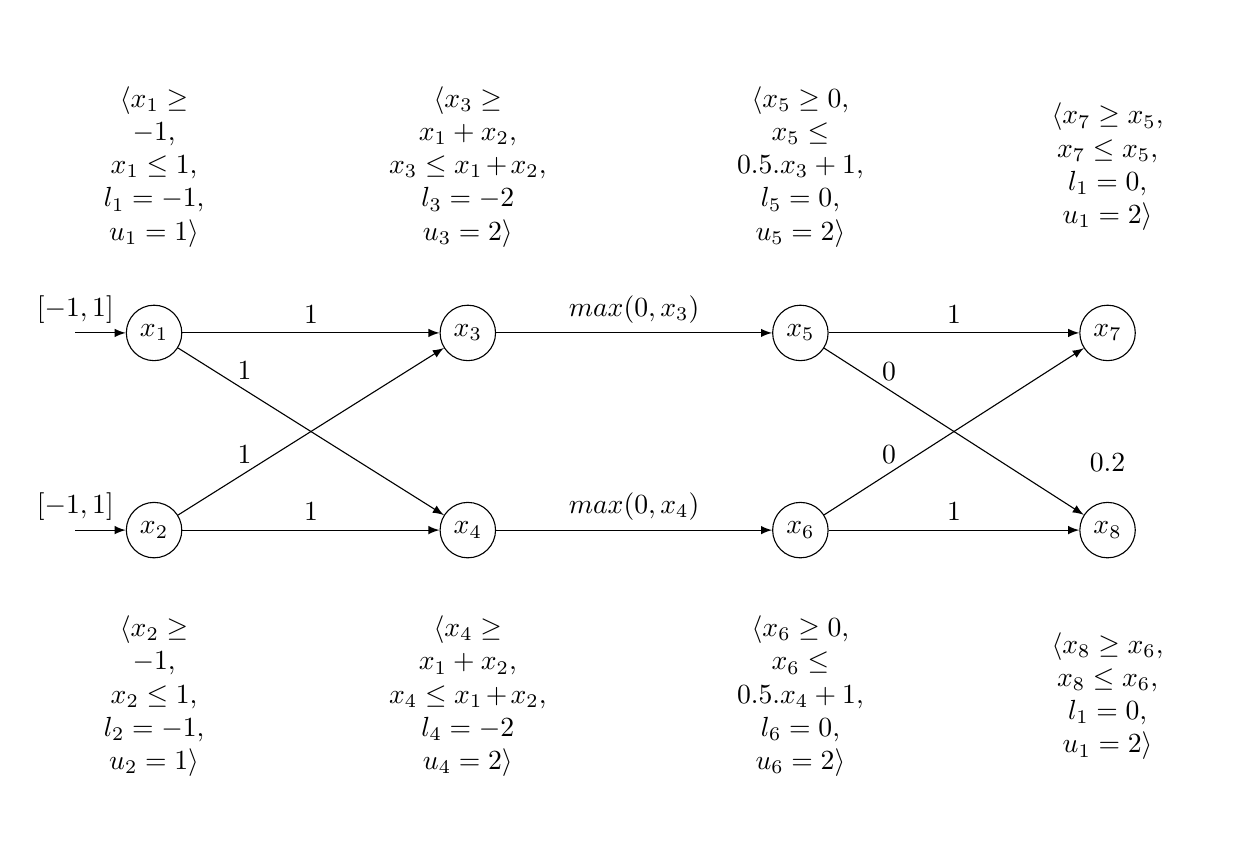
\begin{tikzpicture}[
    % define styles 
    clear/.style={ 
        draw=none,
        fill=none
    },
    net/.style={
        matrix of nodes,
        nodes={ draw, circle, inner sep=3pt },
        nodes in empty cells,
        column sep=1cm,
        row sep=.1cm
    },
    >=latex
]
% define matrix mat to hold nodes
% using net as default style for cells
\matrix[net] (mat)
{
% Define layer headings
   |[clear]| \parbox{1.5cm}{\centering $\langle x_1 \geq -1$, \\ $x_1 \leq 1$, \\ $l_1 = -1$, \\ $u_1 = 1 \rangle$} 
   & |[clear]| \parbox{2cm}{\centering $\langle x_3 \geq x_1 + x_2$, \\ $x_3 \leq x_1 + x_2$, \\ $l_3 = -2$ \\ $u_3 = 2 \rangle$}
   & |[clear]| \parbox{2.2cm}{\centering $\langle x_5 \geq 0$, \\ $x_5 \leq 0.5.x_3 + 1$, \\ $l_5 = 0$, \\ $u_5 = 2 \rangle$}
   & |[clear]|  \parbox{1.5cm}{\centering $\langle x_7 \geq x_5$, \\ $x_7 \leq x_5$, \\ $l_1 = 0$, \\ $u_1 = 2 \rangle$} \\
        
$x_1$  & $x_3$  & $x_5$ & $x_7$ \\
|[clear]| & |[clear]| & |[clear]| & |[clear]| \\
|[clear]| & |[clear]| & |[clear]| & |[clear]| \\
|[clear]| & |[clear]| & |[clear]| & |[clear]| $0.2$ \\
$x_2$  & $x_4$  & $x_6$ & $x_8$ \\
|[clear]| \parbox{1.5cm}{\centering $\langle x_2 \geq -1$, \\ $x_2 \leq 1$, \\ $l_2 = -1$, \\ $u_2 = 1 \rangle$} 
& |[clear]| \parbox{2cm}{\centering $\langle x_4 \geq x_1 + x_2$, \\ $x_4 \leq x_1 + x_2$, \\ $l_4 = -2$ \\ $u_4 = 2 \rangle$}
& |[clear]| \parbox{2.2cm}{\centering $\langle x_6 \geq 0$, \\ $x_6 \leq 0.5.x_4 + 1$, \\ $l_6 = 0$, \\ $u_6 = 2 \rangle$}
& |[clear]| \parbox{1.5cm}{\centering $\langle x_8 \geq x_6$, \\ $x_8 \leq x_6$, \\ $l_1 = 0$, \\ $u_1 = 2 \rangle$} \\
};

% left most lines into input layers
\draw[<-] (mat-2-1) -- +(-1cm,0) node[pos=1, above] {$[-1,1]$};
\draw[<-] (mat-6-1) -- +(-1cm,0) node[pos=1, above] {$[-1,1]$};

\draw[->] (mat-2-1) -- (mat-2-2) node[pos=0.5, above] {$1$};
\draw[->] (mat-2-1) -- (mat-6-2) node[pos=0.25, above] {$1$};
\draw[->] (mat-6-1) -- (mat-2-2) node[pos=0.25, above] {$1$};
\draw[->] (mat-6-1) -- (mat-6-2) node[pos=0.5, above] {$1$};

\draw[->] (mat-2-2) -- (mat-2-3) node[pos=0.5, above] {$max(0,x_3)$};
\draw[->] (mat-6-2) -- (mat-6-3) node[pos=0.5, above] {$max(0,x_4)$};

\draw[->] (mat-2-3) -- (mat-2-4) node[pos=0.5, above] {$1$};
\draw[->] (mat-2-3) -- (mat-6-4) node[pos=0.25, above] {$0$};
\draw[->] (mat-6-3) -- (mat-2-4) node[pos=0.25, above] {$0$};
\draw[->] (mat-6-3) -- (mat-6-4) node[pos=0.5, above] {$1$};


%\draw[->] (mat-2-4) -- +(1cm,0) node[pos=1, above] {$[0,3]$};
%\draw[->] (mat-6-4) -- +(1cm,0) node[pos=1, above] {$[-2,2]$};



% lines from a_{i}^{1} to a_{0}^{2}
%\foreach \ai in {1,2}
%  \draw[->] (mat-\ai-2) -- (mat-6-3);
   
% right most line with Output label
%\draw[->] (mat-6-3) -- node[above] {Output} +(2cm,0);
\end{tikzpicture}
}
	\caption{Hypothetical example of neural network}
	\label{fig:motivating}
\end{figure}
Consider a neural network in figure~\ref{fig:motivating},  which has one input, one hidden, and one output layer. The hidden layer is separated into two layers 
\affine{} and \relu{} layers, so a total of four layers is shown in figure~\ref{fig:motivating}. 
Every layer contains two neurons. The neuron $x_8$ has a bias of $1$ and all the other neurons have a bias of $0$. 
Our goal is to verify for all input $x_1,x_2 \in [-1,1]$ the outputs satisfy $x_7 \leq x_8$. 
Our approach extends \deeppoly{}~\cite{singh2019abstract}. \deeppoly{} maintains the one upper and one lower constraint
as well as upper and lower bound for each neuron. For a neuron of the affine layer, the upper and lower constraint is 
the same, which is the weighted sum of the input neurons i.e. $x_3$'s upper and lower constraint is $x_1+x_2$.
For an activation neuron, the upper and lower expression is computed using triangle approximation~\cite{singh2019abstract}, 
which is briefly explained in section~\ref{sec:deeppoly}. To verify the property $x_7 \leq x_8$, \deeppoly{} creates a 
new expression $x_9 = x_7 - x_8$ and computes the upper bound of $x_9$. The upper bound of $x_9$ should not be greater
than $0$. \deeppoly{} computes the upper bound of $x_9$ by back substituting the expression of $x_7$ and $x_8$ 
from the previous layer.%, the back substitute further from the previous layer.
They continue back substituting until only input layer variables are left.
The process of back substitution is shown in equation (1). %~\ref{eq:deeppoly}.
After back substitution, the upper bound of $x_9$ is
computed as $1$, which is greater than $0$, 
hence, the \deeppoly{} fails to verify the property.

\hspace*{-1cm}
\fbox{
\noindent\begin{minipage}{.23\linewidth}
\begin{equation*}
    \begin{aligned}
        x_9 \leq  &  x_7 - x_8 &\\
        x_9 \leq  & x_5 - x_6 - 1 \\
        x_9 \leq  & 0.5x_3 + 1 - 1 &\\
        x_9 \leq  & 0.5(x_1+x_2) \\
        x_9 \leq  & 1\\
        (1)
   \end{aligned}
%\label{eq:deeppoly}
\end{equation*}
\end{minipage}}\quad
\fbox{
\begin{minipage}{.68\linewidth}
\begin{equation*}
    \begin{aligned}
      -1 \leq & x_1 \leq 1 \hspace*{-1cm}&  \hspace*{-2cm}
      -1 \leq & x_2 \leq 1 \\
         x_1 + x_2 \leq & x_3 \leq x_1 + x_2 \hspace*{-1cm}& \hspace*{-2cm}
         x_1 + x_2 \leq & x_4 \leq x_1 + x_2 \\
         0 \leq & x_5 \leq 0.5x_3+1 \hspace*{-1cm}&  \hspace*{-2cm}
         0 \leq & x_6 \leq 0.5x_4 + 1 \\
         x_5 \leq & x_7 \leq x_5 \hspace*{-1cm}&\hspace*{-2cm}
         x_6+1 \leq & x_8 \leq x_6+1 \\
         x_7 & > x_8 \text{ (negation of property)}&&\\
        & \hspace*{2cm}(2) &&
    \end{aligned}
%\label{eq:conjunction}
\end{equation*}

\end{minipage}
}  

There are two main reasons for the failure of \deeppoly{}. First, it cannot maintain the complete correlation 
between the neurons. In this example neurons $x_3$ and $x_4$ has the same expression $x_1+x_2$, so, they always
get the same value. But in the \deeppoly{} analysis process, it may fail to get the same value. Second, it uses triangle
approximation on relu neurons.
We take the conjunction of upper and lower expressions of each neuron with the negation of the property
as shown in equation (2)%~\ref{eq:conjunction},
 and use the \milp{} solver to check satisfiability, thus addressing the first issue.  
The second issue can be resolved either by splitting the bound at zero of the 
affine node or by using the exact encoding (eq~\ref{eq:reluexact}) 
instead of triangle approximation. 
But both solutions increase the problem size exponentially in terms of relu neurons and this results in a huge 
blowup if we repair every neuron of the network. 

So, the main hurdle towards efficiency is to find the set of important neurons (we call these {\em marked neurons}), 
and only repair these.  For this we crucially use the satisfying assignment obtained from the \milp{} solver.
%When \deeppoly{} fails to verify the network, we use an \milp{} solver to check the satisfiability of equation~\ref{eq:conjunction}. 
%If it returns \unsat{} it means the property is verified otherwise we get the satisfying assignment of each variable. 
For instance, a possible satisfying assignment of equation~(2)%\ref{eq:conjunction}
is in equation~\ref{eq:sat1}. We execute the neural network with the inputs $x_1=1,x_2=1$ and get the values 
on each neuron as shown in equation~\ref{eq:sat2}. 
Then we observe that the output values $x'_7=2, x'_8=3$ satisfy the property, 
so, the input $x_1=1, x_2=1$ is a spurious counterexample. 
The question is to identify the neuron whose abstraction lead to this imprecision.
%\vspace{-20mm}
\setcounter{equation}{2}
\begin{align}
  x_1=1, x_2=1, x_3=2, x_4=2, x_5=2, x_6=0, x_7=2, x_8=1 \label{eq:sat1} \\
  x'_1=1, x'_2=1, x'_3=2, x'_4=2, x'_5=2, x'_6=2, x'_7=2, x'_8=3 \label{eq:sat2}
\end{align}

%We have to remove spurious counter example by doing the refinement analysis. 
%We are using one approach to find the marked neurons guided by the spurious counter example,  and one approach to refine (repair) the marked neurons.

% We are using two approaches to find the marked neurons guided by the spurious counter example, 
% and two approaches to refine (repair) the marked neurons.
% \begin{equation}
%     \begin{aligned}
%         x_1=1, x_2=1, x_3=2, x_4=2, x_5=2, x_6=0, x_7=2, x_8=1\\
%     \end{aligned}
%         \label{eq:sat1}
% \end{equation}

% \begin{equation}
%     \begin{aligned}
%         x'_1=1, x'_2=1, x'_3=2, x'_4=2, x'_5=2, x'_6=2, x'_7=2, x'_8=3
%     \end{aligned}
% \label{eq:sat2}
% \end{equation}


%Following is the approach to find the marked neurons.
%\\
\noindent\textbf{Maxsat based approach to identify marked neurons}\\
%The satisfying assignments of equation~\ref{eq:conjunction} are in equation~\ref{eq:sat1}. We execute the satisfying assignment $x_1=1,x_2=1$ on the neural network and get values on each neuron as  shown in equation~\ref{eq:sat2}.
% We make the point on \texttt{relu} layer in eq~\ref{eq:sat1} as close as possible to the point 
% of \texttt{relu} in equation~\ref{eq:sat2} by encoding them as soft constraints (i.e.,  $\{x_5=2, x_6=2\}$) 
% while maintaining that the rest of the hard constraints are satisfied (see Equation~\ref{eq:opt1})
% e.g., input points $x_1,x_2$ and output points $x_7,x_8$ are the same etc. 
% %The soft constraints define the closeness point on the relu layer of equations~\ref{eq:sat1} and \ref{eq:sat2}. 
% Then we feed this to a maxsat solver \todo{check! afzal} to maximize the soft constraints, 
% while maintaining the hard constraints.
%   %the constraints in equation~\ref{eq:opt1} and the soft constraints. 
% %The constraints of equation~\ref{eq:opt1} must be satisfied because it is the same equation as \ref{eq:conjunction} except for the fixed input and output points. The optimizer returns the constraints from soft constraints which are satisfied with the constraints of equation~\ref{eq:opt1}.
%   If the solver returns all soft constraints($\{x_5=2,x_6=2\}$) it means the output point $x_7=2, x_8=1$ 
%   can be reached from $x_5=2,x_6=2$. But in this case the solver could return only the soft constraint 
%   $\{x_5=2\}$, which implies that $x_6$ is a neuron which is contributing to the output point $x_7=2, x_8=1$. 
%   We mark the neuron $x_6$ as a marked neuron. \todo{this should be written better. maybe the schematic picture should be here for THIS example not general.}
To find the neurons whose abstraction leads to imprecision, let us see figure~\ref{fig:pictorial1}. 
Here, the black line represents the spurious counterexample denoted by equation~\ref{eq:sat1}. 
The green line represents the exact execution of the input point of spurious counterexample 
which is denoted by equation~\ref{eq:sat2}. 
Our goal is to make the black line as close as possible to the green line from the first layer to the last layer, but the 
first and last points should remain the same i.e., $x_1=1,x_2=1,$ and $x_7=2, x_8=1$, the closest line is the blue line.
Here the closeness measures in terms of the equality of the neurons. 
The green and black points are the same for the input layer, i.e., $[1,1]$. On the first affine layer, $l_1$ 
also, the black point $v_1$ is the same as the green point $v'_1$ since the affine layer does not introduce any spurious information. 
For $l_2$, we try to make $v''_2$ close to $v'_2$, such that $v''_2$ reaches to the $v_3$. We do that by encoding 
them as soft constraints (i.e.,  $\{x_5=2, x_6=2\}$) 
while maintaining that the rest of the hard constraints are satisfied (see Equation~\ref{eq:opt1})
e.g., input points $v_0=v''_0$ and output points $v_3=v''_3$ remain same. 
We mark the neurons of the layer where the blue line starts diverging from the green line, i.e., $l_2$. 
The divergence we find by the \maxsat{} query. If \maxsat{} returns all the soft constraints as satisfied, it means
the blue point becomes equal to the green point. If \maxsat{} returns partial soft constraints as satisfied, 
we mark the neurons whose soft constraints are not satisfied. In our example, \maxsat{} returns 
soft constraints $\{x_5=2\}$, soft constraint of $x_6$ could not satisfied, so, we mark $x_6$.
The blue and black lines are the same for our motivating example since it contains only one \relu{} layer. 
However, in general, it may or may not same. We are finding the blue line (the closest to the green line) to mark the 
less number of marked neurons. 




\noindent  
\fbox{
    \begin{minipage}{0.5\linewidth}
\begin{equation}
    \begin{aligned}
        x_1 = 1 & \land x_2 = 1 \\
        x_3 = x_1 + x_2 & \land x_4 = x_1 + x_2 \\
        0 \leq x_5 = 0.5x_3 + 1 & \land 0\leq x_6 \leq 0.5x_4 + 1 \\ 
        x_7 = x_5 & \land x_8 = x_6 + 1 \\
        x_7 = 2 & \land x_8 = 1
    \end{aligned}
    \label{eq:opt1}
\end{equation}
\end{minipage}
  }\;\;
  \begin{minipage}{0.42\linewidth}
%\textbf{Refinement} \\
%We have an approach for the refinement named as {\em MILP-based approach}.
Once we have  $x_6$ as the marked neuron, we use an {\em MILP based approach}, and add the exact encoding of the marked neuron ($x_6$) in addition to the constraints in equation (2) %~\ref{eq:conjunction}
and check the satisfiability, now it becomes \unsat{}, hence, the property verified (see Eq. equation~\ref{eq:reluexact} for more details).
%The exact constraint of a $\relu${} neuron is explained in 
\end{minipage}

\begin{figure}[t]
    \centering
    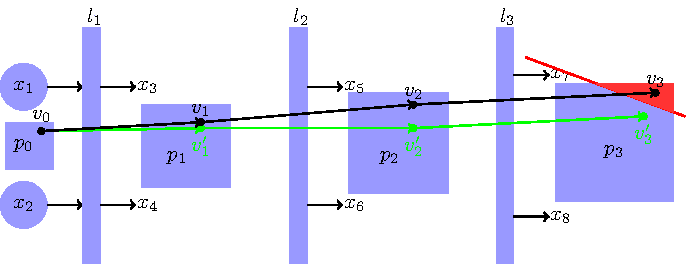
\includegraphics[scale=0.75]{fig/pictorial1.pdf}
    \caption{Pictorial representation of our approach on example in figure~\ref{fig:motivating}}
    \label{fig:pictorial1}
\end{figure}


% \begin{figure}[!ht]
% 	\centering
% 	\scalebox{0.55}{\documentclass[]{standalone}
\usepackage{tikz}
\begin{document}
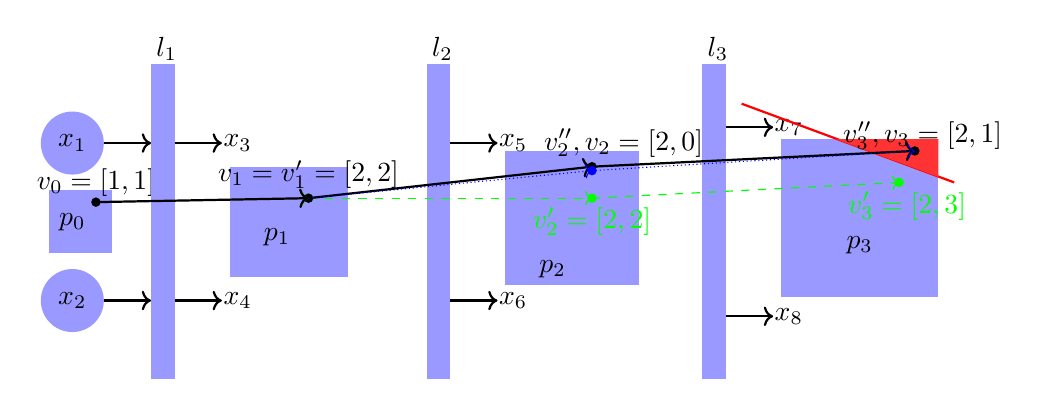
\begin{tikzpicture}
    \fill[blue!40!white] (3,3) circle (4mm);
    \fill[blue!40!white] (3,3) circle (0mm) node[color=black] {$x_1$};
    \fill[blue!40!white] (3,1) circle (4mm);
    \fill[blue!40!white] (3,1) circle (0mm) node[color=black] {$x_2$};
    \fill[blue!40!white] (2.7,1.6) rectangle (3.5,2.4);
    \fill[blue!40!white] (3,2) circle (0mm) node[color=black] {$p_0$};
    \fill[black] (3.3,2.25) circle (.6mm);
    \fill[blue!40!white] (3.3,2.5) circle (0mm) node[color=black] {$v_0 = [1,1]$};
    
    \draw[thick,->] (3.4,3) -- (4,3);
    \draw[thick,->] (3.4,1) -- (4,1);
    \fill[blue!40!white] (4,0) rectangle (4.3,4);
    \fill[blue!40!white] (5,1.3) rectangle (6.5,2.7);
    \fill[blue!40!white] (5.6,1.8) circle (0mm) node[color=black] {$p_1$};
    \draw[thick,->] (4.3,3) -- (4.9,3);
    \draw[thick,->] (4.3,1) -- (4.9,1);
    \fill[blue!40!white] (5.1,3) circle (0mm) node[color=black] {$x_3$};
    \fill[blue!40!white] (5.1,1) circle (0mm) node[color=black] {$x_4$};
    \fill[green] (6,2.3) circle (.6mm);
    \fill[black] (6,2.3) circle (.6mm);
    \fill[blue!40!white] (6,2.6) circle (0mm) node[color=black] {$v_1=v'_1=[2,2]$};
    % \fill[blue!40!white] (6,2) circle (0mm) node[color=green] {$v'_1$};
    \fill[blue!40!white] (4.2,4.2) circle (0mm) node[color=black] {$l_1$};

    \fill[blue!40!white] (7.5,0) rectangle (7.8,4);
    \fill[blue!40!white] (8.5,1.2) rectangle (10.2,2.9);
    \fill[blue!40!white] (9.1,1.4) circle (0mm) node[color=black] {$p_2$};
    \draw[thick,->] (7.8,3) -- (8.4,3);
    \draw[thick,->] (7.8,1) -- (8.4,1);
    \fill[blue!40!white] (8.6,3) circle (0mm) node[color=black] {$x_5$};
    \fill[blue!40!white] (8.6,1) circle (0mm) node[color=black] {$x_6$};
    \fill[green] (9.6,2.3) circle (.6mm);
    \fill[black] (9.6,2.7) circle (.6mm);
    \fill[blue!40!white] (10,3) circle (0mm) node[color=black] {$v''_2,v_2=[2,0]$};
    \fill[blue!40!white] (9.6,2) circle (0mm) node[color=green] {$v'_2 = [2,2]$};
    \fill[blue!40!white] (7.7,4.2) circle (0mm) node[color=black] {$l_2$};


    \fill[blue!40!white] (11,0) rectangle (11.3,4);
    \fill[blue!40!white] (12,1.05) rectangle (14,3.05);
    \fill[blue!40!white] (13,1.7) circle (0mm) node[color=black] {$p_3$};
    \draw[thick,->] (11.3,3.2) -- (11.9,3.2);
    \draw[thick,->] (11.3,.8) -- (11.9,.8);
    \fill[blue!40!white] (12.1,3.2) circle (0mm) node[color=black] {$x_7$};
    \fill[blue!40!white] (12.1,.8) circle (0mm) node[color=black] {$x_8$};
    \draw[red, thick] (14.2,2.5) -- (11.5,3.5);
    \fill[red!80!white] (12.7,3.05) -- (14,2.57) -- (14,3.05) -- cycle;
    \fill[black] (13.7,2.9) circle (.6mm);
    \fill[green] (13.5,2.5) circle (.6mm);
    \fill[blue!40!white] (13.8,3.1) circle (0mm) node[color=black] {$v''_3,v_3=[2,1]$};
    \fill[blue!40!white] (13.6,2.2) circle (0mm) node[color=green] {$v'_3 = [2,3]$};
    \fill[blue!40!white] (11.2,4.2) circle (0mm) node[color=black] {$l_3$};

    \draw[dashed,->,green] (3.3,2.25)  -- (6, 2.3);
    \draw[dashed,->,green] (6,2.3)  -- (9.6, 2.3);
    \draw[dashed,->,green] (9.6, 2.3) -- (13.5, 2.5);

    \draw[thick,->,black] (3.3,2.25)  -- (6, 2.3);
    \draw[thick,->,black] (6,2.3)  -- (9.6, 2.7);
    \draw[thick,->,black] (9.6, 2.7) -- (13.7, 2.9);



    %Following lines are for blue line
    % \draw[thick,->,blue] (3.3,2.25)  -- (6, 2.3);
    \fill[blue] (9.6,2.65) circle (.6mm);
    \draw[densely dotted,->,blue] (6,2.3)  -- (9.6, 2.65);
    \draw[densely dotted,->,blue] (9.6, 2.65) -- (13.7, 2.9);
    % \fill[blue!40!white] (9.9,2.6) circle (0mm) node[color=blue] {$v''_2 = [2,0]$};

\end{tikzpicture}

\end{document}
}
% 	\caption{Pictorial representation of our approach}
% 	\label{fig:pictorial}
% \end{figure}





%% \begin{figure}
%%     \begin{minipage}{0.9\textwidth}
%%         \centering
%%         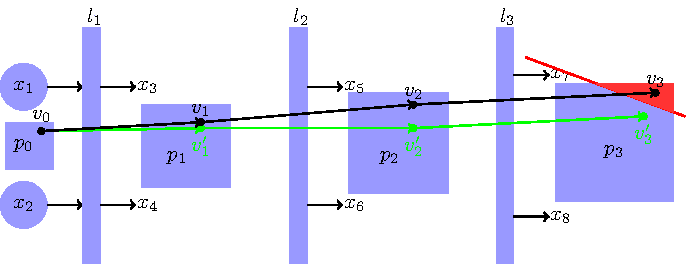
\includegraphics[scale=0.8]{fig/pictorial1.pdf}
        
%%         (a)
%%     \end{minipage}

%%     \begin{minipage}{0.9\textwidth}
%%         \centering
%%         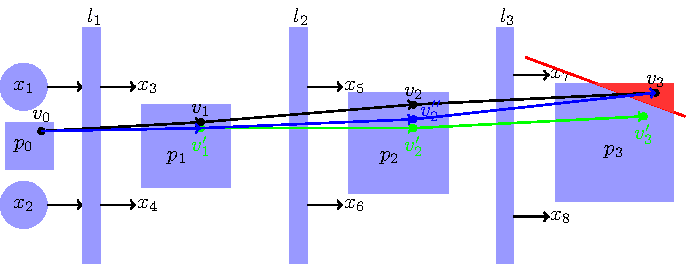
\includegraphics[scale=0.8]{fig/pictorial2.pdf}

%%         (b)
%%     \end{minipage}
%%     \caption{Pictorial representation of our approach}
%%     \label{fig:pictorial}
%% \end{figure}


%% Consider the pictorial representation of our approach in figure~\ref{fig:pictorial}. This pictorial representation is not 
%% related to the motivating example of figure~\ref{fig:motivating}. The shapes $p_0, p_1, p_2$, and $p_4$ represent 
%% the abstract constraints on each layer. We took the rectangle shape for simplicity,  but it is not necessarily a rectangle shape. 
%% The red zone on the output layer shows the intersection of the abstract constraints and the negation of the property. If this 
%% intersection is empty, we can say that the property was verified. Otherwise, we will get a path 
%% $v_0\rightarrow v_1\rightarrow v_2\rightarrow v_3$ as shown in figure~\ref{fig:pictorial}(a), which may or may not be a counterexample. 
%% We execute $v_0$ on neural network
%% and get path $v_0\rightarrow v'_1\rightarrow v'_2\rightarrow v'_3$ as shown in figure~\ref{fig:pictorial}(a). 
%% If the point $v'_3$ reaches the red zone, 
%% we report $v_0$ as a counterexample. Otherwise, we refine the path $v_0\rightarrow v_1\rightarrow v_2\rightarrow v_3$. 
%% To refine, we make the black line close to the green line from the first layer to the last layer so that the endpoints($v_0, v_3$)
%% remain unchanged. Here the closeness means making the neuron's values equal. 
%% First, we make the points $v_1$ close to $v'_1$, and it become completely equal (all neuron's values of $v_1$ become equal to the 
%% corresponding neuron's values of $v'_1$), we move on the the layer $l_2$. 
%% On layer $l_2$,
%% we make the points $v_2$ close to $v'_2$, and some neurons of $v_2$ become equal to the corresponding neurons of $v'_2$, and some
%% neurons could not become equal, so we got a new point $v''_2$ close to $v'_2$.  
%% Finally we got the path $v_0\rightarrow v'_1\rightarrow v''_2\rightarrow v_3$ in figure~\ref{fig:pictorial}(b) 
%% close to the green line.
%% We pick the layer where the blue line diverges first from the green line. Furthermore, get the neurons whose values are different 
%% from the green point's neuron's values. In figure ~\ref{fig:pictorial}(b), the first layer where blue line diverges from the 
%% green line is $l_2$.
%% We find all the neurons of points $v''_2$ and $v'_2$ whose values differ and mark them.     


% \begin{equation}
%     \begin{align}
%         \text{softConstrs} = \{x_5=2, x_6=0\}
%     \end{align}
% \end{equation}


%%% Local Variables:
%%% mode: latex
%%% TeX-master: "../main"
%%% End:


\section{Preliminaries}
\label{sec:model}
%We define the notions and definitions in this section. 
These notions and definitions are used in the later part of the paper. 
The network is defined in the definition \ref*{def:net}. 

% l_{in}, l_{out}
\begin{df}
    \label{def:net}
    A neural network $N = (Neurons, Layers, Edges, W, B, LayerType)$ is a tuple, where
    \begin{itemize}
        \item $Neurons$ is the set of neurons in $N$,
        \item $Layers = \{l_0,...,l_k\}$ is an indexed partition of $Neurons$,
        % \item $l_i \in Layers$ represents the $i^{th}$ layer in network $N$. 
        % \item $|l_i|$ represents the number of neurons in layer $l_i$. 
        % \item 
        \item $ Edges \subseteq \Union_{i=1}^{k} l_{i-1} \times l_{i}$
        \item $W : Edges \mapsto \reals$
        \item $B : Neurons \mapsto \reals$
        \item $LayerType : Layers \mapsto \{\mathtt{Affine}, \mathtt{Relu}\}$
    \end{itemize}
\end{df}

A neural network is a collection of layers $l_0, l_1, l_2, ... l_k$, where $k$ represents the number of layers.
We call $l_0$ and $l_k$ the {\em input} and {\em output layers} respectively, and all the other layers 
as {\em hidden layers}. We assume a separate layer for activation function. Though there are different kinds of
activation, but we focus only on \relu{}, hence each layer can either be an affine layer or an \relu{} layer.
There is a one to one mapping between an affine layer $l_{i-1}$ and a \relu{} layer $l_i$. 
% If a layer $l_i$ is \relu{} layer, then the input neuron of $n_{ij}$ will only be the neuron $n_{(i-1)j}$. 
Let us say a vector $\boldsymbol{val_i} = [val_{i0}, val_{i1}, ... val_{im}]$ represents the values of each neuron 
in the layer $l_i$, where $m$ is the number of nodes in the same layer.
The value of $\boldsymbol{val_i}$ computed by the weighted sum of the previous layer's values($W_i * V_{i-1} + B_i$)
if $l_i$ is affine layer, otherwise $\boldsymbol{val_i}$ computed by the \relu{} function. 
A function $y = max(0,x)$ is a \relu{} function which takes an arguments $x$ as input and return the
same value $x$ as output if $x$ is non-negative otherwise return the value 0. 

A neural network can be visualize as a function $N$ which takes an input of $m$ dimensions and gives an 
output of $n$ dimensions. $N$ can be represented as a composition of functions $f_k o f_{l-1} ... o f_1$,
where each function $f_i$ represents either the linear combinations of previous layer's
output or an activation function. Let us say $n_{ij} \in N.Neurons$ represents 
the $i^{th}$ neuron of layer $l_j$, and $x_{ij}$ is a real variable for $n_{ij}$. 

% For any vector $\boldsymbol{v}$, $v_i$ represents it's $i^{th}$ value.  

% Let $\reals$ be the set of real numbers.
% Let $x_{\alpha}$ are unbounded set of real variables, where
% $\alpha$ is arbitrary index for variables.

\begin{df}
    \label{def:linexpr}
    $Linexpr = \{ w_0 + \sum_{i} w_i x_i | w_i \in \reals \land x_i \text{ is a real variable} \}$.
\end{df}
  
\begin{df}
    \label{def:linconstr}
    $Linconstr = \{expr \text{ op } 0 | expr \in LinExpr \land op \in \{\leq, = \}\}$
\end{df}






\begin{df}
  A matrix $W_i \in \reals^{|l_i|\times|l_{i-1}|}$ represents the weight matrix for layer $l_i$, where  
    $$
    W_i[t_1, t_2] = 
    \begin{cases}
      W(e) & e=(n_{(i-1)t_2}, n_{it_1}) \in Edges,\\
      0 & \text{otherwise.}\\
    \end{cases}
    $$
\end{df}

\begin{df}
    A matrix $B_i \in \reals^{|l_i|\times 1}$ represents the bias matrix for layer $l_i$. The entry $B_i[t,0] = B(n_{it})$, where $n_{it} \in Neurons$. 
\end{df}



\subsection{DeepPoly}
\label{sec:deeppoly}
We develop our abstract refinement approaches on top of \texttt{DeepPoly}
abstraction~\cite{deeppoly}, which is an abstraction-based method.
The abstraction uses the combination of
well understood polyhedra~\cite{polyhedra} and box~\cite{boxd} abstract domain.
The abstraction maintains
upper and lower linear expressions
as well as
upper and lower bounds for each neurons.
The variables appearing in upper and lower expressions are only from
the predecessor layer.\todo{Add some intuition}
Formally, we define the abstraction as follows. 
% Globally \texttt{DeepPoly} forms a polyhedron.
% Experimentally, it has better precision in comparison to Box~\cite{} and Zonotope~\cite{}.
% Deeppoly has the abstract transformer of various types of layers and activation functions.

\begin{df}
    For a neuron $x \in N.neurons$,
    an abstract constraint $A(x) = (lb,ub, lexpr, uexpr)$ is a tuple, where
    $lb \in \reals$ is lower bound on the value of $x$,
    $ub \in \reals$ is the upper bound on the value of  $x$,
    $lexpr \in LinExpr$ is the expression for the lower bound, and
    $uexpr \in LinExpr$ is the expression for the upper bound.
\end{df}

% The abstract constraint $A$ is generated by the tool deeppoly~\cite{} as explained in subsection~\ref*{sec:deeppoly}. 

In \texttt{DeepPoly}, we compute the abstraction $A$ as follow:
\begin{itemize}
\item For an affine neuron $x_{ij}$, we set 
  $A(x_{ij}).lexpr := A(x_{ij}).uexpr := \sum_{t=1}^{|l_{i-1}|} W[j,t]*x_{(i-1)t} + B_i[j,0]$.
  They compute the value of $A(x_{ij}).lb$ and $A(x_{ij}).ub$ by back substituting
  the variables in $A(x_{ij}).lexpr$ and $A(x_{ij}).uexpr$ respectively up to input layer.  
\item For a relu neuron $x_{ij} = max(0,x_{(i-1)j})$, we consider three cases:
            \begin{enumerate}
                \item If $A(x_{(i-1)j}).lb \geq 0$ then relu is in active phase and $A(x_{ij}).lexpr = A(x_{ij}).uexpr = x_{(i-1)j}$,
                        and $A(x_{ij}).lb = A(x_{(i-1)j}).lb$ and $A(x_{ij}).ub = A(x_{(i-1)j}).ub$
                \item If $A(x_{(i-1)j}).ub \leq 0$ then relu is in passive phase and $A(x_{ij}).lexpr = A(x_{ij}).uexpr = 0$, 
                        and $A(x_{ij}).lb = A(x_{ij}).ub = 0$
                \item  If $A(x_{(i-1)j}).lb < 0$ and $A(x_{(i-1)j}).ub > 0$ then the behavior of relu is uncertain, and authors
                        do over-approximation. $A(x_{ij}).uexpr = u(x_{(i-1)j} - l) / (u - l)$, 
                        where $u = A(x_{(i-1)j}).ub \text{ and } l = A(x_{(i-1)j}).lb$.
                        And $A(x_{ij}).lexpr = \lambda . x_{(i-1)j}$, where $\lambda \in \{0,1\}$. 
                        They are choosing the value of $\lambda$ dynamically. They compute the value of $A(x_{ij}).lb$ and $A(x_{ij}).ub$ 
                        by back substituting the variables in $A(x_{ij}).lexpr$ and $A(x_{ij}).uexpr$ respectively up to input layer. 
            \end{enumerate} 
\end{itemize}

The constraints for an affine neuron are exact because it is just an affine transformation of input neurons. 
The constraints for a relu neuron is also exact if relu is either in active or passive phase. 
The constrains for relu is over-approximated if the behavior of relu is uncertain, although the exact 
constraints for this case exist, but with the cost of efficiency. 
The equation ~\ref{eq:reluexact} shows the exact constraints
for a relu neurons when its behavior is uncertain. Let us say the relu neuron is $x_{ij} = max(0,x_{(i-1)j})$. 

\begin{align}
    \label{eq:reluexact}
    \begin{split}
        x_{ij} &\leq x_{(i-1)j} - l*(1-a) \\
        x_{ij} &\geq x_{(i-1)j} \\
        x_{ij} &\leq u*a \\
        x_{ij} &\geq 0 \\
        a &\in \{0,1\} \\ 
        \text{where }l = A(x_{(i-1)j}).lb &\text{ and }u = A(x_{(i-1)j}).ub \\
    \end{split}
\end{align}


\subsection{Solver}


%%% Local Variables:
%%% mode: latex
%%% TeX-master: "main"
%%% End:



% \clearpage

\section{Algorithm}
\label{sec:algo}
In this section, we present our method to refine \deeppoly{}. \deeppoly{} is a sound and incomplete technique because it does over-approximations. If \deeppoly{} verifies the property then the property is guaranteed to be verified, otherwise, its result is unknown. We overcome this limitation by using a CEGAR-like technique, which is complete. In our refinement approach, we mark some \relu{} neurons to have exact behavior on top of~\deeppoly{} constraints, similar to the strategy of refinement in the most complete state-of-the-art techniques~\cite{wang2021beta,xu2020fast}. We add the encoding of the exact behavior to the~\deeppoly{} constraints and use an \milp{} solver on the extended constraints to check if the extra constraints rule out all spurious counterexamples. The calls to MILP solvers are expensive, therefore we use the spurious counterexamples discovered to identify as small as possible set of marked neurons which suffice to be repaired. %\todo{do we need this para at all? seems repetitive.. move this to intro?}

\subsection{The top level algorithm}
\label{sec:toplevelalgo}
We start by describing Algorithm~\ref{algo:main}, where we present the top-level flow of our approach. 
The algorithm takes a verification query $\langle N,P,Q \rangle$ as input, where $N$ is a neural network and $P,Q$ are predicates over input and output layers respectively, and returns success if the verification is successful.
Otherwise it returns a counterexample to the query. The algorithm uses supporting algorithms $\textsc{getMarkedNeurons}$ and 
$\textsc{isVerified}$ (described subsequently) to get more marked neurons to refine and check the validity of the verification query  after refinement.


The first line of the algorithm performs preprocessing steps similar to state-of-the-art tools (e.g. \alphabeta{}). These preprocessing steps are optional and are explained in more detail in Section~\ref{sec:experiments}, where they are used to compare our results with those of state-of-the-art tools. The fourth line of Algorithm~\ref{algo:main} generates all the abstract constraints by using \deeppoly{},  as described in Section~\ref{sec:deeppoly}.  For a node $n_{ij} \in N.neurons$, the abstract constraints consist of the lower and upper constraints as well as the lower and upper bounds. 
Let $A.lc_i = \Land_{j=1}^{|l_i|} A(n_{ij}).lexpr \leq x_{ij} \leq  A(n_{ij}).uexpr$, which is a conjunction of upper and lower 
constraints of each neuron of layer $l_i$ with respect to abstract constraint $A$. 
The $lexpr$ and $uexpr$ for any neuron of a layer contain variables only from the previous layer's neurons, hence $A.lc_i$ contains the variables from layers $l_{i-1}$ and $l_i$. If the preprocessing steps in line 1 are applied, then \deeppoly{} generates the $lexpr$ and $uexpr$ for \relu{} neurons as per the triangle approximation. In this case, we may return a counter-example and stop or use these bounds without performing any back-substitution. 

% If the bounds provided in the \deeppoly{} call at line number $4$ are tighter than vanilla \deeppoly{} \todo{what is the vanilla deeppoly?} then it keeps the 
% tighter bounds and generate the $lexpr$ and $uexpr$ accordingly. \todo{why is this not written in the algo itself?}

% We start by describing Algorithm~\ref{algo:main}, where we present the top-level flow of our approach. The algorithm takes a verification query $\langle N,P,Q \rangle$ as input and returns success if the verification is successful, otherwise returns a counterexample to the query. The algorithm uses supporting algorithms $\textsc{getMarkedNeurons}$ and $\textsc{isVerified}$ (described subsequently) to get more marked neurons to refine and check the validity of the verification query after refinement.

% The first line of Algorithm~\ref{algo:main} generates all the abstract constraints by using \deeppoly{}, as described in Section~\ref{sec:deeppoly}. For a node $n_{ij} \in N.neurons$, the abstract constraints consist of the lower and upper constraints as well as the lower and upper bounds. Let $A.lc_i = \Land_{j=1}^{|l_i|} A(n_{ij}).lexpr \leq x_{ij} \leq  A(n_{ij}).uexpr$, which is a conjunction of upper and lower constraints of each neuron of layer $l_i$ with respect to abstract constraint $A$. The $lexpr$ and $uexpr$ for any neuron of a layer contain variables only from the previous layer's neurons, hence $A.lc_i$ contains the variables from layers $l_{i-1}$ and $l_i$. 




\begin{algorithm}[t]
  \textbf{Input: } A verification problem $\langle N,P,Q \rangle$ \\
  \textbf{Output: } UNSAT or SAT
  \begin{algorithmic}[1]
    \State $\mathsf{cex}, bounds = preprocessing(N,P,Q)$
    \If{cex is not None}
      \State \textbf{return} Failed(cex)
    \EndIf
    \State $A := \deeppoly{(N,P, bounds)}$\Comment{use \deeppoly{} to generate abstract constraints.}
    \State $marked$ := \{\}
    \While{True}
      \State result = $\textsc{isVerified}$($\langle N,P,Q \rangle$, $A$, $marked$)
      \If{result = CEX(${v_0}, {v_1} ... {v_k}$)}
        \If{$N({v_0}) \models \lnot Q$}
          \State \textbf{return} Failed(${v_0}$)
        \Else
        \State $markedNt$ := $\textsc{getMarkedNeurons}$($N$, $A$, $marked$, ${v_0}, {v_1} ... {v_k}$)
          \State $marked$ := $marked$ $\union$ $markedNt$
        \EndIf
      \Else
        \State \textbf{return} verified
      \EndIf
    \EndWhile
  \end{algorithmic}
  \caption{A CEGAR based approach of neural network verification}
  \label{algo:main}
\end{algorithm}
\begin{algorithm}[t]
  \textbf{Name: } $\textsc{isVerified}$ \\
  \textbf{Input: } Verification query $\langle N,P,Q \rangle$, abstract constraints $A$, $marked \subseteq ~ N.neurons$ \\
  \textbf{Output: } verified or an abstract counterexample. 
  \begin{algorithmic}[1]
    \State $constr := P \land (\Land_{i=1}^k A.lc_i)\land \neg Q$
    \State $constr := constr \land (\Land_{x \in marked} exactConstr(x))$ \Comment{as in eq \ref*{eq:reluexact}}
    \State isSat = checkSat(constr)
    \If{isSat}
      \State m := getModel(constr)
      \State \textbf{return} CEX($m(x_0),....,m(x_k)$)
    \Else
      \State \textbf{return} verified
    \EndIf
  \end{algorithmic}
  \caption{Verify $\langle N,P,Q \rangle$ with abstraction A}
  \label{algo:verif1}
\end{algorithm}

\begin{algorithm}[t]
  \textbf{Name: } $\textsc{getMarkedNeurons}$ \\
  \textbf{Input: } Neural network $N$, \deeppoly{} abstraction $A$, $marked\subseteq N.neurons$, and abstract counterexample $({v_0}, {v_1} ... {v_k})$\\
  \textbf{Output: } New marked neurons. 
  \begin{algorithmic}[1]
    % \State \textbf{return} ${x}$ if $N({x}) \models \neg Q$. 
    \State Let ${val^{v_0}_{ij}}$ be the value of $n_{ij}$, when ${v_0}$ is input of $N$. 
    \For{$i=1$ to $k$} \Comment{inputLayer excluded}
      \If{$l_i$ is $\relu${} layer}
        \State $constr := \Land_{t=i}^k A.lc_t$
        \State $constr := constr \land (\Land_{n \in marked} exactConstr(n))$ \Comment{as in eq \ref{eq:reluexact}}
        \State $constr := constr \land \Land_{j=1}^{|l_{i-1}|} (x_{(i-1)j} = val^{v_0}_{(i-1)j})$
        \State $constr := constr \land \Land_{j=1}^{|l_k|} (x_{kj} = v_{kj})$
        \State $softConstrs := \cup_{j=1}^{|l_j|} (x_{ij} = val^{v_0}_{ij})$
        \State $res, softsatSet = \maxsat{}(constr, softConstrs)$ \Comment{res always \sat{}}
        \State $newMarked := \{n_{ij} | 1 \leq j \leq |l_i| \land (x_{ij} = val_i(j)) \notin  softsatSet\}$ 
        \If{$newMarked$ is empty}
          \State \textbf{continue}
        \Else
          \State \textbf{return} $newMarked$
        \EndIf 
      \EndIf
    \EndFor
  \end{algorithmic}
  \caption{Marked neurons from counterexample}
  \label{algo:refine2}
\end{algorithm}
% \todo{what is N.neurons? should it be Neurons? Answer ashu: N is neural network. N.neurons is the set of neurons}

At line 5, we initialize the variable $marked$ to the empty set of neurons.  At the next line, we iterate in a while loop until 
either we verify the query or find a counterexample. At line 7, we call $\textsc{isVerified}$ with the verification query, 
abstraction $A$, and the set of marked neurons. In this verification step, the behavior of the marked neurons is encoded exactly, 
as detailed in Section~\ref{sec:verif}. The call either returns that the query is verified or returns an abstract counterexample, 
which is defined as follows.

% At line 2, we initialize the variable $marked$ to the empty set of neurons.  At the next line, we iterate in a while loop until either we verify the query or find a counterexample. At line 4, we call $\textsc{isVerified}$ with the verification query, abstraction $A$, and the set of marked neurons. In this verification step, the behavior of the marked neurons is encoded exactly, as detailed in Section~\ref{sec:verif}. The call either returns that the query is verified or returns an abstract counterexample, which is defined as follows.

\begin{df}
  A sequence of value vectors ${v_0}, {v_1}, ... , {v_k}$ is an 
  {\em abstract execution} of abstract constraint $A$ if 
  ${v_0} \models lc_0$ and ${v_{i-1}}, {v_i} \models A.lc_i$ for each $i \in [1,k]$.  
  An abstract execution ${v_0,...,v_k}$ is
  an {\em abstract counterexample} if~${v_k} \models \lnot Q$.
\end{df}

If these algorithms return verified, we are done, otherwise we analyze the abstract counterexample $CEX(v_0,...,v_k)$.
At line 8, we first check if executing the neural network $N$ on input $v_0$
violates the predicate $Q$.
If yes, we report input $v_0$ for which the verification query is not true.
Otherwise, we declare the abstract counterexample to be spurious.
We call $\textsc{getMarkedNeurons}$ to analyze the counterexample and
return the cause of spuriousness, which is a set of neurons $markedNt$.
We add the new set $markedNt$ to the old set $marked$ and iterate our loop with the new set of marked neurons. Now let us present $\textsc{isVerified}$ and $\textsc{getMarkedNeurons}$ in detail.

% Algorithm \ref{algo:verif1} exploits the markedNeurons to verify the property. 

%
% The algorithm uses supporting algorithms~\ref{algo:refine1} and~\ref{algo:verif1} to
% verify the query and return either the verification successful or abstractCEX. 

% The algorithm~\ref{algo:main} represents the high-level flow of our approach.



% Our approach contains two parts, the first part contains an approach to finding the markedNeurons. 
% The second part contains the verification approach (utilizing markedNeurons).


% In algorithm ~\ref{algo:refine2} and ~\ref{algo:verif1}
% They are presented in 

% \clearpage

% The goal is to find an input ${x}$, such that the predicates $P({x})$ and 
% $Q(N({x}))$ holds. The predicate $Q$ usually is the negation of the desired property. 
% The triple  is our verification query.
%  \todo{How to formalize $P$ and $Q$}

% An input vector ${v} \in \reals^{|l_0|}$ is a counterexample(cex) if $N({v}) \models \lnot Q$. 
% Let us say $satval_{ij}$ represents the satisfying value of variable $x_{ij}$, after an optimization query. 


% We will use the following convention in writing our algorithms.


% \begin{itemize}
% \item 
% \item 
% % \item $W_i, B_i$ represent the weight and bias matrix of layer $l_i$ respectively. 
% \end{itemize}


% \begin{df}
% \end{df}






\subsection{Verifying query under marked neurons}
\label{sec:verif}
In Algorithm~\ref{algo:verif1}, we present the implementation of 
$\textsc{isVerified}$, which takes the verification query, the \deeppoly{} abstraction $A$,
and a set of marked neurons as input.
At line 1, we construct constraints $contr$ that encodes the executions that satisfy abstraction
$A$ at every step.
At line 2, we also include constraints in $constr$ that encodes the exact behavior of the marked
neurons. The following is the encoding of the exact behavior~\cite{tjeng2017evaluating} of neuron $n_{ij}$.
\begin{align}
    \label{eq:reluexact}
    \begin{split}
      exactConstr(n_{ij}) := x_{(i-1)j} \leq x_{ij} &\leq x_{(i-1)j} - A(n_{(i-1)j}).lb*(1-a) \;\;\land  \\
        0 \leq x_{ij} &\leq A(n_{(i-1)j}).ub*a \land a \in \{0,1\} \\ 
    \end{split}
\end{align}
where $a$ is a fresh variable for each neuron.

At line 3, we call a solver to find a satisfying assignment of the constraints.
If $constr$ is satisfiable, we get a model $m$.
From the model $m$, we extract an abstract counterexample and return it.
If $constr$ is unsatisfiable, we return that the query is verified.


% \subsection{Causes of spuriousness}

% We have a following approach to find the causes of spuriousness (markedNeurons). 

\subsection{Maxsat based approach to find the marked neurons}
\label{sec:markedneurons}
In Algorithm~\ref{algo:refine2}, we present $\textsc{getMarkedNeurons}$
which analyzes an abstract spurious counterexample.
In our abstract constraints, we encode $\affine${} neurons exactly, but
over-approximate $\relu${} neurons.
We identify a set of
marked neurons whose exact encoding will eliminate the counterexample
in the future analysis.
%
%
As we defined earlier, let ${val_i^{{v_0}}}$ represent the value vector
on layer $l_i$, if we execute the neural network on input ${v_0}$.
%
Let us say ${v_0}, {v_1}, ... ,{v_k}$ is an abstract spurious counterexample.
We iteratively modify the counterexample such that its values coincides with ${val_i^{{v_0}}}$.
Initially, ${val_0^{{v_0}}}$ is equal to $v_0$.
Since we encode the affine layer exactly in $A.lc_i$, the following
theorem follows.

% % 
% ${v_0}$ is a counterexample if ${val_k^{{v_0}}}$ 
% does not satisfy the property $Q$.

\begin{theorem}
  \label{th:marked2}
  Let ${v_0}, {v_1}, ... {v_k}$ be an abstract execution. For all $1\leq i\leq k$, if $Type_i = \affine$ and ${val_{i-1}^{{v_0}}} = {v_{i-1}}$, then ${val_i^{{v_0}}} = {v_i}$.
\end{theorem}
% \begin{proof}
%   Since affine layer's constraints are exact.
% \end{proof}
% Since $l_0$ is an input layer, so, ${v_0}$ and ${val_0^{v_0}}$ are equal,

By the above theorem, ${v_1}$ and ${val_1^{v_1}}$ are also equal. 
The core idea of our algorithm is to find ${v'_2}$ as close as possible to ${val_2^{v_0}}$, 
such that ${v_0}, {v_1}, {v'_2}, ... {v'_{k-1}}, {v_k}$ becomes an abstract spurious counterexample. 
We measure closeness by the number of elements of ${v'_2}$ are equal to the 
corresponding element of vector ${val_2^{v_0}}$.
\begin{enumerate}
\item If ${v'_2}$ is equal to ${val_2^{v_0}}$ then ${v'_3}$ will also become 
  equal to ${val_3^{v_0}}$ due to Theorem \ref{th:marked2}. 
  Now we move on to the next $\relu${} layer $l_4$ and try to find the similar point ${v'_4}$, such that 
  ${v_0}, {v_1}, {v_2}, {v_3},{v''_4}... {v''_{k-1}},{v_k}$ is an abstract spurious counterexample. 
  We repeat this process until the following case occurs. 
\item If at some $i$, we can not make ${v'_i}$ equal to ${val_i^{v_0}}$ then we collect the neurons
  whose values are different in ${v'_i}$ and ${val_i^{v_0}}$. We call them marked neurons.
\end{enumerate}

In the algorithm, the above description is implemented using \maxsat{} solver.
The loop at line 2 iterates over $\relu${}~layers.
In lines 4-7, we build constraints that encode that from layer $i$ onward
\deeppoly~abstract constraints are satisfied,
the marked neurons have exact behavior, layer $(i-1)$ neurons have value equal to
${val_{i-1}^{v_0}}$, and the execution finishes at $v_k$.
At line 8, we construct soft constraints $softConstrs$, which encodes $x_{ij}$ is equal to $val_{i}^{v_0}$.
At line 9, we call \maxsat{} solver. 
This call to \maxsat{} solver will always find a satisfying assignment because
our hard constraints are always satisfiable.
The solver will also return a subset $softsatSet$ of the soft constraints.
At line 10, we check which soft constraints are missing in $softsatSet$.
The corresponding neurons are added in $newMarked$.
If $newMarked$ is empty, we have managed to find a spurious
abstract counterexample from $val^{v_0}_{i}$ and we go to the next layer.
Otherwise, we return the new set of marked neurons.

%% \begin{figure}
%%   \centering
%%   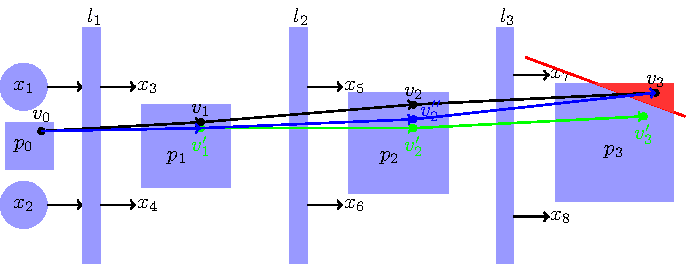
\includegraphics[scale=0.55]{fig/pictorial2.pdf}
%%   \caption{Pictorial representation of our approach}
%%   \label{fig:pictorial}
%% \end{figure}

% \subsection{Utilizing of spurious information}
% The \emph{isVerified} function in algorithm~\ref{algo:main} calls algorithm~\ref{algo:verif1}. 
% The algorithm~\ref{algo:verif1} takes \markednewrons{} as input. 
% The \markednewrons{} represent the set of the culprit neurons. 
% Algorithm~\ref{algo:verif1} replaces the abstract constraints of \markednewrons{} by exact constraints and check for the 
% property by \milp{} solver. If \milp{} solver return \sat{} then we return satisfying assignments as an abstractCEX, 
% otherwise, return verified. 
















%--------------------- DO NOT ERASE BELOW THIS LINE --------------------------

%%% Local Variables:
%%% mode: latex
%%% TeX-master: "../main"
%%% End:



%\section{Variations}
%\label{sec:variations}
% \begin{figure}[t]
    \centering
    \begin{tikzpicture}[level/.style={sibling distance=60mm/#1}]
        \node(g){$\globally$} child {node (u) {$\until$} child {node (s) {$\varphi(2)$} child[dashed, gray]
            {node[draw, circle, minimum size=0.3cm, gray] (l) {} child
            {node[draw, circle, minimum size=0.3cm, gray] (ll) {}} child
            {node[draw, circle, minimum size=0.3cm, gray] (lr) {}}}
            child[dashed, gray] {node[draw, circle, minimum size=0.3cm] (r) {}
            child {node[draw, circle, minimum size=0.3cm, gray] (rl)
            {}} child {node[draw, circle, minimum size=0.3cm, gray]
            (rr) {}}}} child {node
            (x) {$x$}}};
    \end{tikzpicture}
    \caption{Example subtree construction for Hybrid Pattern Matching}
\label{fig:subtree}
\end{figure}

We have presented a scheme of ranking formulae and an algorithm to find the best
formula ranked on a trace.
%
However, our scheme has many possibilities of variations. For example, the
choice of various constants and relative importance of LTL operators is one
such. 
%
In this section, we will discuss a couple of variations.
% \sankalp{Possibly an example involving several equally scored formulae? Thread
% locking? th1\_wait U $\neg$ lock, as well as th2\_wait U $\neg$ lock?}

\emph{Hybrid Pattern Matching: }
The algorithm as defined in  sections \ref{sec:cso} and \ref{sec:opm} suffers
from a certain common drawback, though at different ends of the spectrum.
%
Otherwise, we can always discover more and more complex formulae.
%
The issue is further enhanced by the constraint sizes growing far too  quickly
with increase in the depth of the pattern. 

In the case of  \emph{pattern matching}, the algorithm does not check a large
enough variety of properties (it is guided by the template pattern) and, for the
same reason,  is also quite \emph{insufficiently} expressive in comparison with
constrained system optimization. 
%
To remedy this, we allow a middle ground, where, instead of attempting to learn
formulae from scratch or from explicit patterns, we allow learning
\emph{subformulae} within some known patterns.
%
A subformulae argument $\varphi(n)$ with $n$ being a prescribed maximum depth for
the subtree can be provided as part of the pattern, parsed into the tree as an
abstracted empty formula with constraints constructed for the specified nodes
explicitly, and for the subformulae recursively in the manner as described for
seciton \ref{sec:cso}. In Figure \ref{fig:subtree}, we show an example of the
hybrid pattern $\globally (\varphi(2) \: \until \: x)$, where $\varphi(2)$ is an
unknown formula of depth less than $2$ and $x$ is an unknown letter.

\begin{algorithm}
    \begin{algorithmic}[1]
        \Procedure{HybridPattern}{$P, N, pattern$} \Comment{Returns optimal
            formula fitting a pattern}
        
            \State \textbf{parse} pattern 
            \State construct $\varphi^{\var}_\prop$ for propositional patterns in tree
            \State construct $\varphi^{ST}_\textnormal{n}$ for every subformula pattern $\varphi(n)$ in the tree
            \State constraint $\Phi \leftarrow \varphi^{\var}_\prop \land \bigwedge \varphi^{ST}_\textnormal{n}$
            \State optimize
            $\min( \{y_{0,0}^\tau\: |\: \tau \in P\} )$ with $\Phi$ as constraint
            
            \If{optimization succeeds with model m} \Comment SAT \State
                construct formula tree from m \State \textbf{return}
                optimized formula tree \Else \State \textbf{return} UNSAT \EndIf
                \EndProcedure
    \end{algorithmic}
    \caption{Computing the optimal formula given a partial pattern}
    \label{algo:hybrid}
\end{algorithm}

\emph{Prioritize variables: }
%
In case there is a large set of events and we want bias the focus of our search
towards certain letters in the traces that do not occur very often, we may
adjust the value $V(p,w)$ assigned to each propositional variable $p$.
%
In our default scheme, we assign $V(p,w) = 1$ if $w(1)$ contains $p$.
%
A user may assign a value greater than $1$ to variables $p$ that are desirable
and assign less than $1$ for the variables $p$ that are not.
% %
% As a variation of Optimized Pattern Matching, we let the user to fix a subset
% of  variables to appear in the pattern and compute the best mapping of the
% other variables per specification.
%
This allows for mining specifications pertaining to the prioritized variables in
cases where several competing well ranked specifications are present.
%
Let $\pi$ be the map from the propositional variables $\prop$ to their priority.
%
We replace equation~\eqref{eq:prop_score} by the following formula where we
return score $\pi(p)$ instead of $1$. 
% %
% To achieve this, in addition to~\eqref{eq:map}, the following
% constraint~\eqref{eq:fixed} is added, which binds the common variable to
% itself.
% %
% \begin{align} \bigwedge _{p \in Var \intersection \prop} m_{p, p}
%     \label{eq:fixed} \end{align}

\begin{align}
    \bigwedge _{1 \leq i \leq N} \bigwedge _{p \in \prop} x_{i, p} \rightarrow \left[ 
        \bigwedge _{1 \leq t \leq |\tau|} y^\tau _{i, t} = \begin{cases}
            \pi(p) & \textnormal{if } p \in \tau (t) \\
            0 & \textnormal{if } p \not \in \tau (t)
        \end{cases}
    \right] \label{eq:prop_priority_score} 
\end{align}

Recall that we considered the trace in figure~\ref{fig:exampletrace}, where we
wanted to find a property $\globally \:\texttt{auth\_failed}\: \Leftrightarrow\:
\varphi(1)$. We may further abstract the property $\globally \: \varphi(0) \:
\Leftrightarrow\: \varphi(1)$ by setting the priority map $\pi =
\{\texttt{auth\_failed} \mapsto 10, otherwise \mapsto 1\}$. We obtain the same
result from \ourtool.

% Of course, the best mapping for $x$ is $\texttt{connected}$ and the tool
% returns the formula $\globally (\texttt{connected} \until
% \texttt{disconnected})$. 

The above variations suggest that our method is viable to be adapted  to an
application at hand, where we want to bias our ranking to give preference to a
desired class of formulae.


% --- no delete below this line --

%%% Local Variables:
%%% mode: latex
%%% TeX-master: "main"
%%% End:


%\clearpage
\section{Experiments}
\label{sec:experiments}
% We have implemented our approach in a prototype and compared it three types of related approaches (i) \deeppoly{}~\cite{singh2019abstract} and its refinements \texttt{kPoly}~\cite{singh2019beyond}, \texttt{deepSRGR}~\cite{yang2021improving}, (ii) other cegar based approaches and 
%The approaches  \texttt{kPoly} and \texttt{deepSRGR} do the refinement on \deeppoly{}.
(iii) state-of-the-art tools \alphabeta~\cite{alphabetacrown} and \ovaltool~\cite{ovaltool}, both of which use a set/portfolio of different algorithms and optimizations. The first tool~\alphabeta{} achieved the 1st and \ovaltool{} 3rd rank in the 2nd International Verification of Neural Networks Competition (VNN-COMP'21).
%We use the MNIST \cite{deng2012mnist} for our evaluation.    
\subsection{Implementation}
We have implemented our techniques in a tool, which we call \drefine{}, in \texttt{C++} programming language. Our approach relies on \deeppoly{}, so we also have implemented \deeppoly{} in \texttt{C++}. We are using a \texttt{C++} interface of the tool Gurobi~\cite{?} \todo{add ref} to check the satisfiability as well as solve  \texttt{maxsat} queries. %We have implemented our technique as a tool and call it \drefine{}.  

\subsection{Benchmarks}
We use the MNIST~\cite{deng2012mnist} dataset to check the effectiveness of our tool and comparisons. We are using 11 different fully connected feedforward neural networks with $\relu${} activation as shown in table~\ref{tb:nndetail}.
These benchmarks are taken from the \deeppoly{}'s paper~\cite{singh2019abstract}.  The input and output dimensions of each network are $784$ and $10$ respectively. 
The authors of \deeppoly{} used projected gradient descent (PGD)~\cite{dong2018boosting}
and DiffAI~\cite{mirman2018differentiable} for adversarial training. Table \ref{tb:nndetail} contains the defended network i.e.
trained with adversarial training as well as the undefended network. The last column of the table \ref{tb:nndetail} how the defended networks were trained.  

The predicate $P$ on the input layer is created using the input image $\boldsymbol{im}$ and user-defined parameter $\epsilon$.  We first normalize each pixel of $\boldsymbol{im}$ between $0$ and $1$, then create  $P = \Land_{i=1}^{|l_0|} im(i)-\epsilon \leq x_{0i}\leq im(i)+\epsilon$, such that the lower and upper bound of each pixel should not exceed $0$ and $1$ respectively. The predicate $Q$ on the output layer is created using the network's output.     Suppose the predicted label of $\boldsymbol{im}$ on network $N$ is $y$, then $Q = \Land_{i=1}^{|l_k|} x_{ki} < y$, where $i \neq y$.  One query instance $\langle N,P,Q \rangle$ is created for one network, one image and one epsilon value.  In our evaluation, we took $11$ different networks, 8 different epsilons, and 100 different images. The 
total number of instances is $8800$. However, there are 128 instances for which the network's predicted label differs from the image's actual label. we avoided such instances, so, there is a total of $8672$ benchmark instances
under consideration.    Whenever our tool found a counter-example on $\langle N,P,Q \rangle$, it denormalizes it into an image by rounding the float values 
and checks for counter-example by executing $N$ on the denormalized image.
If a counter-example is found then the tool reports it, otherwise, the tool reports unknown.



\begin{table}[t]
    \centering
    \begin{tabular}{c|c|c|c}
        \hline
        \textbf{Neural Network} & \textbf{\#hidden layers} & \textbf{\#activation units} & \textbf{Defensive training} \\
        \hline
        $3\times 50$ & 2 & 110 & None \\
        $3\times 100$ & 2 & 210 & None  \\
        $5\times 100$ & 4 & 410 & None  \\
        $6\times 100$ & 5 & 510 & DiffAI \\
        $9\times 100$ & 8 & 810 & None  \\
        $6\times 200$ & 5 & 1010 & None  \\
        $9\times 200$ & 8 & 1610 & None  \\
        $6\times 500$ & 6 & 3000 & None  \\
        $6\times 500$ & 6 & 3000 & PGD, $\epsilon = 0.1$ \\
        $6\times 500$ & 6 & 3000 & PGD, $\epsilon = 0.3$ \\
        $4\times 1024$ & 3 & 3072 & None  \\
        \hline
    \end{tabular}
    \caption{Neural networks details}
    \label{tb:nndetail}
\end{table}

\subsection{Results}
We conducted the experiments on a machine with \texttt{64GB RAM, 2.20 GHz Intel(R) Xeon(R) CPU E5-2660 v2}
processor with CentOS Linux 7 operating system. 
To make a fair comparison between the tools, we provide only a single \texttt{CPU} for each instance for each tool. 
We make three types of comparisons as shown in (i) Figure~\ref{res:milp_with_milp}, which is a cactus plot of (log of) time taken vs the number of benchmarks solved (ii) Table~\ref{tb:matrix}, which makes a pairwise comparison of the number of instances that a tool could solve which another couldn't  (more precisely, the $(i,j)$-entry of the table is the number of instances which could be verified by tool $i$ but not by tool $j$) and (iii) Figure~\ref{res:ep:milp_with_milp} which compares wrt epsilon, the robustness parameter.
%represents the verified cases while the column represents the not verified cases, i.e.\kpoly{}'th row and \deeppoly{}'th column represent the  156 number of benchmarks instances which are solved by \kpoly{} and not solved by \deeppoly{}. 

We remark that on an average, \drefine{} marks $9.8\%$ of neurons, whenever it needs to refine.  \todo{probably should be moved somewhere else?}

\subsubsection{Comparison with the most related techniques:}
In this subsection, we consider the techniques \deeppoly{}, \kpoly{}, and \deepsrgr{} to compare with our technique. 
We consider \deeppoly{} because it is at the base of our technique, and the techniques \kpoly{} and \deepsrgr{} refine \deeppoly{} just as we do. These tools only report \texttt{verified} instances, while our tool can report  \texttt{verified} and the counter-example. We note that we compare these techniques with only \texttt{verified}  instances of our technique in the line of \texttt{drefine\_verified} in cactus plot ~\ref{res:milp_with_milp}. 

It can be seen that our technique outperforms the others in terms of the verified number of instances. One can also see that when they do verify, \deeppoly{} and \kpoly{} are efficient compared to our tool which is not surprising, while our tool is more efficient than \deepsrgr{}. From Table~\ref{tb:matrix}, we also see  that our tool solves all the benchmark instances which are solved by these three techniques (and significantly more ~3700 for the first two and ~1000 for the third), except $14$ instances where \kpoly{} succeeds and our tool times out.

% The approaches \deeppoly{}, \texttt{refinepoly}, and \texttt{deepSRGR} are incomplete and do not report the counter-example. 
% Our approach is a complete approach. We compare our approach's \texttt{verified} only instances with incomplete approaches. 
% Figure~\ref{res:milp_with_milp} shows the comparison with the help of the cactus plot. Our approach performs well 
% in terms of the verified number of instances as well as in terms of time in comparison to the above incomplete approaches. 
% We are also comparing with state of the arts to check the effectiveness of our approach globally.
% Table~\ref{tb:soacomparison} shows that our tool is verifying $180$ and $190$ benchmarks which $\alpha -\beta$-CROWN and 
% \texttt{oval} respectively are not able to verify. In addition to this, our tool verifies $172$ unique instances 
% that neither $\alpha -\beta$-CROWN nor \texttt{oval} is able to verify.  
% Despite it, $\alpha - \beta-$Crown and \texttt{oval} are verifying more benchmarks in comparison to our tool. 
% Although the total time taken by both state of the arts is higher than our tool as shown in figure~\ref{res:milp_with_milp}. 


% \begin{table}
%     \centering
%     \begin{tabular}{|c|c|c|c|}
%         \hline
%         -  & Not verified by oval & Not verified by $\alpha - \beta$-CROWN & Not verified by both \\
%         \hline
%         Verified by our tool & 190 & 180 & 172 \\
%         \hline
%     \end{tabular}
%     \caption{Comparison with $\alpha - \beta$-CROWN and Oval}
%     \label{tb:soacomparison}
% \end{table}



\begin{figure}[t]
  % \centering
  
\begin{tikzpicture}
    \begin{axis}[
        xlabel={Number of benchmarks},
        ylabel={log(time)},
        width=13cm,
        height=9cm,
        xmin=0, xmax=7000,
        ymin=0, ymax=25,
        xtick={0,1000,2000,3000,4000,5000,6000,7000},
        ytick={0,5,10,15,20,25},
        legend pos=south east,
        legend entries={drefine, deeppoly, deep\_SRGR, refinepoly, drefine\_verified, alpha\_beta, oval, cegar\_nn},
        ymajorgrids=true,
        xmajorgrids=true,
        grid style=dashed,
    ]
    \addplot[
        color=blue
    ] 
    table {fig/drefine_data.txt};
    
    \addplot[
        color=red
    ] 
    table {fig/deeppoly_data.txt};

    \addplot[
        color=orange
    ] 
    table {fig/deepsrgr_data.txt};

    \addplot[
        color=green
    ] 
    table {fig/refinepoly_data.txt};

    \addplot[
        color=violet
    ]
    table {fig/drefine_verified_data.txt};
    
    \addplot[
        color=purple
    ]
    table {fig/alpha_beta_data.txt};

    \addplot[
        color=brown
    ]
    table {fig/oval_data.txt};

    \addplot[
        color=gray
    ]
    table {fig/four_class_data.txt};

    \end{axis}

\end{tikzpicture}
  \caption{Cactus plot with related techniques}
  \label{res:milp_with_milp}
\end{figure}

\subsubsection{Comparison with cegar based techniques: }
\texttt{cagar\_nn}~\cite{elboher2020abstraction} is a tool that also uses  counter example guided refinement~\todo{afzal, in intro we also refer to arxiv paper. should we remove that?}. But the abstraction used is quite different in comparison to the  \deeppoly{}. This tool reduces the size of the network by merging the similar neurons, such that they maintain the overapproximation and split back in the refinement process. We can see in Figure~\ref{res:milp_with_milp} that \texttt{cegar\_nn} could verified only  $18.88\%$ while our tool verified $61.42\%$ of the total number of benchmark instances. Although, in total \texttt{cegar\_nn} solves significantly fewer benchmarks, it is pertinent to note that this technique solves many unique benchmark instances as can be inferred from Table~\ref{tb:matrix}. Again this shows the orthogonal nature of this technique compared to the others.% the tool \texttt{cegar\_nn} is deployed completely different technique in comparison to others. 


\subsubsection{Comparison with portfolio state of the arts: }
The tools \alphabeta{} and \ovaltool{} use several algorithms that are highly optimized and could even be considered as portfolio solvers. The authors of \alphabeta{} implement the techniques~\cite{alphabetapapers}\todo{afzal, cite all papers here}, and the authors of \ovaltool{} implement~\cite{ovalpapers}
Figure~\ref{res:milp_with_milp} shows that both the tools indeed solve about 1000 (out of 8000) more than we do. However, we found around $180$ benchmarks instances where \alphabeta{} fails and our tool works. Also, around $190$ benchmarks on which \ovaltool{} fails and our tool works; see table~\ref{tb:matrix} for more details. In total, we are solving $172$ unique benchmarks where both tools fail to solve. Thus we believe that these tools are truly orthogonal in their strengths and could potentially be combined. We also note that in terms of total time, both tools are taking more time in comparison to our tool. 

\begin{figure}[t]
%    \centering
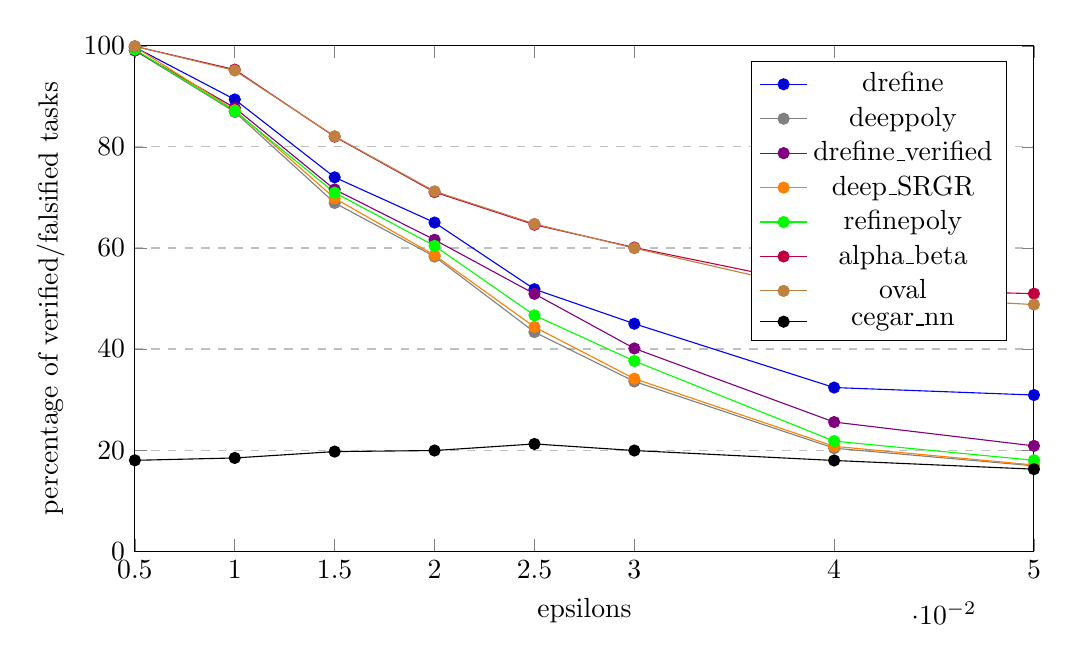
\begin{tikzpicture}
    \begin{axis}[
        xlabel={epsilons},
        ylabel={percentage of verified/falsified tasks},
        width=13cm,
        height=8cm,
        xmin=0.005, xmax=0.05,
        ymin=0, ymax=100,
        xtick={0.005,0.01,0.015,0.02,0.025,0.03,0.04,0.05},
        ytick={0,20,40,60,80,100},
        legend pos=north east,
        legend entries={drefine,deeppoly, drefine\_verified, deep\_SRGR, refinepoly, alpha\_beta, oval, cegar\_nn},
        ymajorgrids=true,
        grid style=dashed,
    ]
    \addplot+[
        color=blue,
        mark=*,
    ]
    coordinates {
        (0.005,99.72)(0.01,89.39)(0.015,73.98)(0.02,65.03)(0.025,51.84)(0.03,45.01)(0.04,32.38)(0.05,30.9)
    };

    \addplot[
        color=gray,
        mark=*,
    ]
    coordinates {
        (0.005,99.07)(0.01,86.9)(0.015,68.91)(0.02,58.3)(0.025,43.35)(0.03,33.58)(0.04,20.38)(0.05,16.89)
    };

    \addplot[
        color=violet,
        mark=*,
    ]
    coordinates {
        (0.005,99.07)(0.01,87.73)(0.015,71.58)(0.02,61.62)(0.025,50.92)(0.03,40.12)(0.04,25.55)(0.05,20.84)
    };

    \addplot[
        color=orange,
        mark=*,
    ]
    coordinates {
        (0.005,99.8)(0.01,87.26)(0.015,69.83)(0.02,58.57)(0.025,44.37)(0.03,34.13)(0.04,20.75)(0.05,17.06)
    };

    \addplot[
        color=green,
        mark=*,
    ]
    coordinates {
        (0.005,99.26)(0.01,87.08)(0.015,70.94)(0.02,60.42)(0.025,46.67)(0.03,37.63)(0.04,21.78)(0.05,17.99)
    };

    \addplot[
        color=purple,
        mark=*,
    ]
    coordinates {
        (0.005,99.9)(0.01,95.29)(0.015,82.02)(0.02,71.05)(0.025,64.60)(0.03,60.09)(0.04,51.98)(0.05,50.96)
    };

    \addplot[
        color=brown,
        mark=*,
    ]
    coordinates {
        (0.005,99.9)(0.01,95.11)(0.015,82.1)(0.02,71.21)(0.025,64.76)(0.03,59.96)(0.04,50.92)(0.05,48.8)
    };

    \addplot[
        color=black,
        mark=*,
    ]
    coordinates {
        (0.005,17.98)(0.01,18.45)(0.015,19.71)(0.02,19.92)(0.025,21.22)(0.03,19.92)(0.04,17.95)(0.05,16.23)
    };


    \end{axis}

\end{tikzpicture}
    \caption{Size of input perturbation (epsilon) vs. percentage of solved instances}
    \label{res:ep:milp_with_milp}
\end{figure}


\begin{table}[b]
  \footnotesize
    \centering
    \begin{tabular}{|c|c|c|c|c|c|c|c|c|}
        \hline
      - & \textbf{total} & \textbf{cegar\_} & \textbf{deeppoly} & \textbf{kPoly} & \textbf{deepSRGR} & $\alpha \beta-$ & \textbf{oval} & \textbf{drefine} \\
        &     & \textbf{\_nn}& & & & \textsc{CROWN}& & \\
        \hline
        \textbf{cegar\_nn} & 1638 & 0 & 713 & 609 & 687 & 217 & 238 & 417 \\ 
        \hline
        \textbf{deeppoly} & 4633 & 3708 & 0 & 0 & 0 & 63 & 66 & 0  \\ 
        \hline
        \textbf{kPoly} & 4789 & 3760 & 156 & 0 & 114 & 63 & 66 & 14  \\ 
        \hline
        \textbf{deepSRGR} & 4687 & 951 & 54 & 2 & 0 & 63 & 66 & 0 \\ 
        \hline
        \alphabeta{} & 6242 & 4821 & 1672 & 1516 & 1618 & 0 & 84 & 1095  \\
        \hline
        \textbf{Oval} & 6189 & 4789 & 1622 & 1466 & 1568 & 31 & 0 & 1052 \\
        \hline
        \textbf{drefine} & 5327 & 4106 & 694 & 552 & 640 & 180 & 190 & 0  \\
        \hline
    \end{tabular}
    \caption{Comparison of tools, example row \kpoly{} and column \deeppoly{} represents 156 benchmark instances on which \kpoly{} but \deeppoly{} fails}
    \label{tb:matrix}
\end{table}

\subsubsection{Epsilon vs. performance: }
For sanity check, we analyzed the effect of perturbation size and the performance of the tools.
In Figure~\ref{res:ep:milp_with_milp}, we present the comparison of fractional success rate of tools as the size of epsilon values grow from $0.005$ to $0.05$. 
At $\epsilon=0.005$, the performance of all the tools is almost the same. As the value of epsilon increases, the success rate of the the tools drop consistently.
Here also, we are performing better than the approaches \deeppoly{}, 
\texttt{kPoly}, \texttt{deepSRGR} and \texttt{cegar\_nn}, while \alphabeta{} and \ovaltool{} perform better.

% Figures \ref{res:milp_with_milp} and \ref{res:ep:milp_with_milp} shows that we are performing better in compare to
% the most related techniques \deeppoly{}, \texttt{refinepoly} and \texttt{deepSRGR}. 


% \todo{recall what is epsilon... x axis label can perhaps be written out more}



%--------------------- DO NOT ERASE BELOW THIS LINE --------------------------

%%% Local Variables:
%%% mode: latex
%%% TeX-master: "../main"
%%% End:




\section{Conclusion and Future work}
\label{sec:conclusion}
%We have presented a novel cegar-based approach, which results in a scalable and efficient approach.  
Our approach comprises two parts. One part finds the causes of spuriousness, 
while the other parts refine  the information found in the first part. 
Experimental evaluation shows that we outperform related refinement techniques, in terms of efficiency and effectivity. 
We are also verify several benchmarks that are beyond state of the art solvers, highly optimized solvers.
As futurework, we plan to extend our technique/tool to make it independent of \deeppoly{} and applicable with other 
abstraction based techniques and tools. %We believe this could lead to more benchmarks being solved overall.
 %Such that we can improve the results on top of the state of the arts.  


\bibliographystyle{unsrt}
\bibliography{biblio}

%\appendix

%% \onecolumn

\begin{center}
    \Large{\bf{Appendix}}    
\end{center}

\section{Experiments}
\subsection{Comparison with PGD's adversarially trained network}
\label{ap:exp:1}

The networks considered for evaluation in this study are the ones corresponding to the 9th, and 10th 
rows of Table~\ref{tb:nndetail}. These networks have been trained using adversarial techniques, 
where adversarial examples were generated using PGD attack, and the network was subsequently 
trained on these adversarial examples to enhance its robustness. Table~\ref{tb:matrix2} presents a 
pairwise comparison of verifiers on these adversarially trained networks, 
encompassing a total of 1456 benchmark instances. 
Our approach demonstrates significant superiority over \deeppoly{}, \kpoly{}, and \deepsrgr{} in terms of 
performance on these benchmarks. While \alphabeta{} and \ovaltool{} outperform our approach by approximately 
90 benchmarks, we are still able to solve 75 unique benchmarks that remain unsolved by both of these tools. 
Considering the total number of benchmarks is 1456, this indicates a notable number of benchmarks that our 
approach successfully addresses.

\begin{table}[t]
  \scriptsize
    \centering
    \begin{tabular}{|c|c|c|c|c|c|g||c|}
        \hline
        \diagbox{\tiny Verified}{\tiny \mbox{}\hspace{-2mm}Unverified} & \tiny \textbf{\deeppoly} & \tiny \textbf{\kpoly} & \tiny \textbf{\deepsrgr} & \tiny \textbf{\alphabeta} & \tiny \textbf{\ovaltool} & \tiny \textbf{\drefine} & \tiny \textbf{\textsc{total}} \\
        \hline
        \tiny \textbf{\deeppoly} & \textbf{0} & 0 & 0 & 3 & 3 & 0 & 913 \\
        \hline
        \tiny \textbf{\kpoly} & 9 & \textbf{0} & 9 & 5 & 4 & 2 &  922 \\ 
        \hline
        \tiny \textbf{\deepsrgr} & 2 & 2 & \textbf{0} & 3 & 3 & 0 & 915 \\ 
        \hline
        \tiny \textbf{\alphabeta} & 250 & 243 & 250 & \textbf{0} & 1 & 163 & 1160 \\ 
        \hline
        \tiny \textbf{\ovaltool} & 258 & 259 & 258 & 9 & \textbf{0} & 170 & 1168 \\
        \hline
        \rowcolor{green!20}
        \tiny \textbf{\drefine} & 170 & 163 & 168 & 76 & 75 & \textbf{0} & 1073 \\
        \hline
    \end{tabular}
    % \caption{Pairwise comparison of tools on adversarially trained networks, e.g. entry on row \kpoly{} and column \deeppoly{} represents 9 benchmark instances on which \kpoly{} verified but \deeppoly{} fails. The green row highlights the number of solved benchmark instances by \drefine{} and not others while the red column is the opposite.}
    \caption{Pairwise comparison of tools on adversarially trained networks}
    \label{tb:matrix2}
\end{table}





% \subsubsection{Pullback approach: }

% Suppose the abstractCEX is $\boldsymbol{v_0}, \boldsymbol{v_1}, ... , \boldsymbol{v_k}$. 
% The core idea of this approach is to find a point $\boldsymbol{p_{k-1}}$ in the layer $l_{k-1}$. 
% The point $\boldsymbol{v_k}$ is guaranteed to be reachable from point $\boldsymbol{p_{k-1}}$ in the concrete domain.
% Similarly, we find points $\boldsymbol{p_{k-3}}, \boldsymbol{p_{k-5}}, ... \boldsymbol{p_0}$, 
% such that $p_i$ is always reachable from point $p_{i-2}$. 
% We find these points on each $\relu${} layer and input layer only. 
% If we find the point $\boldsymbol{p_0}$ in the input layer, it means $\boldsymbol{p_0}$ is a counter-example, 
% because we can reach from $\boldsymbol{p_0}$ to $\boldsymbol{p_2}$, $\boldsymbol{p_2}$ to $\boldsymbol{p_4}$ 
% , and so on up to $\boldsymbol{v_k}$. 
% If we get stuck in some layer $l_i$ i.e. fails to find point 
% $\boldsymbol{p_{i-2}}$. It means point $\boldsymbol{p_i}$ does not have its corresponding point $\boldsymbol{p_{i-2}}$, 
% which implies that point $\boldsymbol{p_i}$ is a spurious point generated by $\relu${} layer $l_i$. 
% The algorithm \ref{algo:refine1} compute such points. In line number $2$, we equate the value of 
% each element of $\boldsymbol{v_k}$ to the corresponding neuron's affine expression($lexpr$ or $uexpr$), 
% and take the conjunction, and check satisfiability. Since the affine expression of each neuron in $l_k$ contains the 
% variable of layer $l_{i-1}$, so, the satisfying assignment is the point $p_{k-1}$. Similarly, we build the constraints
% for each hidden affine layer's neurons. For a neuron $n_{ij}$ of affine layer $l_i$, 
% if the corresponding point's value $p_{i+1}(j)$ is greater than $0$ then we equate the affine expression of $x_{ij}$ to $p_{i+1}(j)$,
% otherwise, we set the lower and upper bound of the affine expression of $x_{ij}$ as $A(x_{ij}).lb$ and $0$ respectively. 
% Which is the replication of $\relu${} function $x_{(i+1)j} = max(0, x_{ij})$. We construct such constraint 
% for each neuron of $l_i$, and build a formula by taking the conjunction
% of each neuron’s constraint and checking the satisfiability of this formula.
% If it is satisfiable then the point $\boldsymbol{p_{i-1}}$ is found, 
% otherwise, we get the $\mathtt{unsat}$core. We collect all the neurons of $l_i$ whose constraints are 
% in $\mathtt{unsat}$core, and return them as the markedNeurons.   



% \begin{algorithm}[t]
%     \textbf{Name: } pullback \\
%     \textbf{Input: } $\langle N,P,Q \rangle$, abstract constraints $A$ and abstractCEX $=\boldsymbol{v_0}, \boldsymbol{v_1}, .., \boldsymbol{v_k}$ \\
%     \textbf{Output: } markedNeurons or cex. 
%     \begin{algorithmic}[1]
%      \State \textbf{return} $\boldsymbol{v_0}$ if $N(\boldsymbol{v_0}) \models \neg Q$. 
%      \State $constr := \Land_{j=1}^{|l_k|} (A(x_{kj}).lexpr = v_k(j))$
%      \State isSat = checkSat(constr)
%      \If{isSat} \Comment{must be true, last affine layer dont add spurious information}
%         \State $\boldsymbol{p_{k-1}} = \boldsymbol{satval_{k-1}}$ 
%      \EndIf
%      \For{$i=k-1$ to $1$}
%         \If{$l_i$ is affine layer}
%           \State $layerConstraints := true$
%           \For{$j=1$ to $|l_i|$}
%             \If{$p_{i+1}(j) > 0$}
%               \State $constr_{ij}$ := $(A(x_{ij}).lexpr = p_{i+1}(j)$) \Comment{lexpr=uexpr for affine}
%             \Else
%               \State $constr_{ij}$ := $(A(x_{ij}).lb \leq A(n_{ij}).lexpr \leq 0$)
%             \EndIf
%             \State $layerConstrains := layerConstrains \land constr_{ij}$
%           \EndFor
%           \State isSat = checkSat(layerConstrains)
%           \If{not isSat}
%             \State markedNeurons = \{$n_{ij}$ | $1 \leq j\leq |l_i| \land constr_{ij}$ $\in$ unsatCore\}
%             \State \textbf{return } markedNeurons
%           \Else
%             \State $\boldsymbol{p_{i-1}} = \boldsymbol{satval_{i-1}}$
%           \EndIf
%         \EndIf
%      \EndFor
%       \State \textbf{return} $\boldsymbol{p_0}$ \Comment{cex if pullbacked till input layer}
%     \end{algorithmic}
%     \caption{A pullback approach to get mark neurons or counter example}
%     \label{algo:refine1}
%   \end{algorithm}



% \subsection{Utilizing of spurious information}
% The \emph{isVerified} function in algorithm~\ref{algo:main} calls either algorithm~\ref{algo:verif1} or algorithm~\ref{algo:verif2}. 
% Both algorithms~\ref{algo:verif1} and \ref{algo:verif2} take \markednewrons{} as input. 
% The \markednewrons{} represent the set of the culprit neurons. 
% Algorithm~\ref{algo:verif2} splits each neuron of \markednewrons{} into two sub-cases. Suppose the 
% neuron $x\in [lb,ub]$ belongs to \markednewrons{}, then the first case is when $x \in [lb,0]$, and the second case is when $x \in [0,ub]$.   
% After splitting neurons into two cases \deeppoly{} runs for both cases separately. In algorithm \ref{algo:verif2}, \deeppoly{}
% runs an exponential number of times in the size of the \markednewrons{}. We return verified in algorithm~\ref{algo:verif2} if 
% the verification query is verified in all the \deeppoly{} runs. If \deeppoly{} fails to verify in any case then we return the abstractCEX. 

% \begin{algorithm}[t]
%   \textbf{Name: } isVerified2 \\
%   \textbf{Input: } $\langle N,P,Q \rangle$ with abstract constraints $A$ and markedNeurons \\
%   \textbf{Output: } verified or  abstractCEX. 
%   \begin{algorithmic}[1]
%     \For{all combination in $2^{markedNeurons}$}
%       \State $A'$ = run deeppoly
%       \State $constr := P \land (\Land_{i=1}^k lc'_i) \land \neg Q$ \Comment{$lc'$ is with respect to $A'$}
%       \State isSat = checkSat(constr)
%       \If{isSat}
%         \State \textbf{return} abstractCEX
%       \EndIf
%     \EndFor
%     \State \textbf{return} verified
%   \end{algorithmic}
%   \caption{An approach to verify $\langle N,P,Q \rangle$ with abstraction A}
%   \label{algo:verif2}
% \end{algorithm}




% \textbf{Pullback approach}\\
% % The core idea of this approach is to find a point in the predecessor layer, such that the current point 
% % can be reached from the predecessor layers point. 
% This approach finds a point of $x_7=2,x_8=1$ in the predecessor layer means the value of $x_5$ and $x_6$. 
% The point $x_7=2$ and $x_8=1$ must reach from the values of $x_5$ and $x_6$. 
% We compute the value by using the \sat{} query on the affine layer. The \sat{} query shown 
% in equation~\ref{eq:back1}, 
% build by using the values and affine expression of $x_7$, $x_8$, and by using the bounds of $x_5$ and $x_6$.
% The satisfying value of equation~\ref{eq:back1} is $x_5=2$ and $x_6=0$, which is the predecessor point of $x_7=2$
% and $x_8=1$.  
% \begin{equation}
%     \begin{aligned}
%         x_7 = 2 & \land x_8 = 1 \\
%         x_5 = 2 & \land x_6 + 1 = 1 \\ 
%         x_5=2\land x_6+1 = 1 & \land 0\leq x_5 \leq 2 \land 0\leq x_6 \leq 2 \\
%     \end{aligned}
% \label{eq:back1}
% \end{equation}

% In this approach, we compute the predecessor point by considering both the \texttt{affine} and \texttt{relu} layers together. 
% We compute the predecessor point of $x_5=2, x_6=0$ in terms of $x_1$ and $x_2$.
% Since $x_6=0$ and $x_6=max(0,x_4)$ then $x_4$ can be anything from its lower bound to $0$ i.e. $-2 \leq x_4 \leq 0$.
% Similarly the value of $x_5=2$ and $x_5=max(0,x_3)$ then the value of $x_3$ will be $2$. 
% The \sat{} query build as shown in equation~\ref{eq:back2}. 

% \begin{equation}
%     \begin{aligned}
%         x_5 = 2 & \land x_6 = 0 \\
%         x_3 = 2 & \land -2\leq x_4 \leq 0 \\ 
%         x_1+x_2=2\land -2\leq  x_1+x_2 \leq 0 & \land -1\leq x_1 \leq 1 \land -1\leq x_2 \leq 1 \\
%     \end{aligned}
% \label{eq:back2}
% \end{equation}

% When we check the satisfiability of equation~\ref{eq:back2}, it returns \unsat{}. It means the predecessor point of 
% $x_5=2,x_6=0$ does not exist, which implies that point $x_5=2, x_6=0$ is introduced by the triangle approximation.
% Whenever the solver returns \unsat{}, we also get the \unsatcore{}~\ref{sec:solver}. In this example we get the 
% \unsatcore{}=$\{x_1+x_2=2, -2\leq  x_1+x_2 \leq 0\}$, so, we mark the corresponding neurons $x_3$ and $x_4$ as a marked neurons. 
% And refine the marked neurons in the refinement procedure. 


% \textbf{Refinement} \\
% We have two approaches for the refinement {\em Splitting based approach} and {\em MILP-based approach}.
% We elaborate here the {\em MILP-based approach} only. The other approach can be seen in algorithm~\ref{algo:verif2}. 
% These two approaches refine the marked neurons. We got two different sets of marked neurons in the above analysis. 
% The {\em pullback} approach returns $\{x_5, x_6\}$ as the marked neurons, while {\em optimization-based approach}
% return $\{x_6\}$ as the marked neurons. In the following analysis, we are taking the marked neurons set as $\{x_5, x_6\}$.
% Although the analysis will also work if we take the other set of marked neurons.

% In {\em MILP based approach}, we add the exact encoding of the marked neuron ($x_5, x_6$) in addition to the constraints
% in equation~\ref{eq:conjunction} and check the satisfiability, now it becomes \unsat{}, hence, the property verified. 
% The exact constraint of a $\relu${} neuron is explained in equation~\ref{eq:reluexact}. 

% The {\em Splitting based approach} splits the bounds at $0$ of the incoming neurons of the marked neurons. 
% The incoming neurons of $x_5$ and $x_6$ are $x_3$ and $x_4$ respectively. 
% The affine expression of both the incoming neurons is $x_1+x_2$. 
% When we split both $x_3$ and $x_4$ then four cases get generated. The property should get verified in all four cases. 
% All the cases are explained as follows: 
% % Suppose I split $x_3$ then two cases generated
% % $x_3 > 0$ and $x_3 \leq 0$, which implies $x_1+x_2 > 0$ and $x_1+x_2 \leq 0$ respectively. 
% % When we split both $x_3$ and $x_4$ then four cases get generated. Out of four cases $x_3 > 0 \land x_4 \leq 0$ and 
% % $x_3 \leq 0 \land x_4 > 0$ are infeasible cases, because the corresponding affine expression 
% % $x_1+x_2 > 0 \land x_1 + x_2 \leq 0$ is infeasible. We analyze the remaining tow cases as follow: 
% \begin{itemize}
%     \item $x_3 > 0$ and $x_4 > 0$, since neurons are in active phase, so, upper and lower expressions for $x_5$ 
%     becomes $x_3$, similarly the upper and lower expression for $x_6$ becomes $x_4$. 
%     The expression for $x_7$ and $x_8$ remains the same. The upper bound of $x_7 - x_8$ computed in equation~\ref{eq:split1} is $-1$. 
%     The property got verified.   
%     \item $x_3 \leq 0$ and $x_4 \leq 0$, since both neurons are in passive phase, so, the upper and lower expressions 
%         for both the neurons become $0$. The upper and lower expressions of the other neurons remain same. 
%         The upper bound of $x_7 - x_8$ is computed $-1$ in equation~\ref{eq:split2}. The property got verified here too. 
%     \item $x_3 \leq 0$ and $x_4 > 0$, is infeasible case because $x_1+x_2 \leq 0 \land x_1 + x_2 > 0$ is infeasible. 
%     \item $x_3 > 0$ and $x_4 \leq 0$, is infeasible case because $x_1+x_2 > 0 \land x_1 + x_2 \leq 0$ is infeasible. 
% \end{itemize}

% \begin{equation}
%     \begin{aligned}
%         x_7 - x_8 \leq & x_5 - x_6 - 1 \\
%        \leq & x_3 - x_4 -1 \\
%        \leq & x_1 + x_2 -(x_1+x_2) -1 \\
%        \leq & -1 
%     \end{aligned}
%     \label{eq:split1}
% \end{equation}

% \begin{equation}
%     \begin{aligned}
%       x_7 - x_8 \leq & x_5 - x_6 - 1 \\
%         \leq & 0 - 0 - 1 \\
%         \leq & -1
%     \end{aligned}
%     \label{eq:split2}
% \end{equation}




\end{document}

% --- do not erase below this line ----

%%% Local Variables:
%%% mode: latex
%%% TeX-master: t
%%% End:
